\documentclass[11pt,a4paper]{article}

% ---------- Packages ----------
\usepackage[a4paper,margin=2.4cm]{geometry}
\usepackage{amsmath,amssymb,mathtools}
\usepackage{physics}
\usepackage{xcolor}
\usepackage{tcolorbox}
\tcbuselibrary{skins,breakable}
\usepackage{enumitem}
\usepackage{fancyhdr}
\usepackage{titlesec}
\usepackage{listings}
\usepackage{hyperref}
\usepackage{lastpage}
\usepackage{booktabs}
\usepackage{array}
\usepackage{tikz}
\usepackage{multicol}
\usetikzlibrary{decorations.pathreplacing,decorations.pathmorphing,arrows.meta,calc,positioning}

% ---------- Colours ----------
\definecolor{ntccblue}{RGB}{20,60,110}
\definecolor{ntccgold}{RGB}{175,130,20}
\definecolor{boxgrey}{RGB}{245,245,248}
\definecolor{keybg}{RGB}{235,242,250}
\definecolor{probbg}{RGB}{250,244,230}
\definecolor{drawbg}{RGB}{255,255,255}
\definecolor{codebg}{RGB}{40,44,52}
\definecolor{codefg}{RGB}{220,223,228}
\definecolor{pitbg}{RGB}{252,235,238}
\definecolor{histbg}{RGB}{238,248,235}
\definecolor{expbg}{RGB}{240,247,250}

% ---------- Section styling ----------
\titleformat{\section}
  {\normalfont\Large\bfseries\color{ntccblue}}
  {\thesection}{0.6em}{}[{\color{ntccgold}\titlerule[1pt]}]
\titleformat{\subsection}
  {\normalfont\large\bfseries\color{ntccblue}}
  {\thesubsection}{0.6em}{}
\titleformat{\subsubsection}
  {\normalfont\bfseries\color{black}}
  {\thesubsubsection}{0.6em}{}

% ---------- Header/Footer ----------
\pagestyle{fancy}
\fancyhf{}
\renewcommand{\headrulewidth}{0.4pt}
\fancyhead[L]{\small\itshape PH7302E -- Condensed Matter Physics}
\fancyhead[R]{\small\itshape Module 2: Lattice Vibrations \& Thermal Properties --- Student Edition}
\fancyfoot[C]{\small \thepage\ of \pageref{LastPage}}

% ---------- tcolorbox styles ----------
\newtcolorbox{keybox}[1][]{
  colback=keybg, colframe=ntccblue, boxrule=0.6pt, arc=2pt,
  left=6pt, right=6pt, top=4pt, bottom=4pt,
  title={#1}, fonttitle=\bfseries\small, coltitle=white,
  colbacktitle=ntccblue, boxsep=2pt
}
\newtcolorbox{physbox}[1][Physical Picture]{
  colback=boxgrey, colframe=black!50, boxrule=0.4pt, arc=1pt,
  left=6pt, right=6pt, top=4pt, bottom=4pt,
  title={#1}, fonttitle=\bfseries\small\itshape, coltitle=black,
  colbacktitle=white, coltitle=ntccblue, boxsep=2pt
}
\newtcolorbox{probbox}[1][Tutorial / Practice Problems]{
  colback=probbg, colframe=ntccgold!80!black, boxrule=0.5pt, arc=1pt,
  left=6pt, right=6pt, top=4pt, bottom=4pt,
  title={#1}, fonttitle=\bfseries\small, coltitle=white,
  colbacktitle=ntccgold!80!black, boxsep=2pt
}
\newtcolorbox{solbox}[1][Worked Solution]{
  colback=white, colframe=ntccblue!60, boxrule=0.4pt, arc=1pt,
  left=6pt, right=6pt, top=4pt, bottom=4pt,
  title={#1}, fonttitle=\bfseries\small, coltitle=white,
  colbacktitle=ntccblue!60, boxsep=2pt
}
\newtcolorbox{pitbox}[1][Pitfall -- Common confusion]{
  colback=pitbg, colframe=red!55!black, boxrule=0.5pt, arc=2pt,
  left=6pt, right=6pt, top=4pt, bottom=4pt,
  title={\textbf{!}~#1}, fonttitle=\bfseries\small, coltitle=white,
  colbacktitle=red!55!black, boxsep=2pt
}
\newtcolorbox{histbox}[1][Historical note]{
  colback=histbg, colframe=black!50!green!60!black, boxrule=0.4pt, arc=2pt,
  left=6pt, right=6pt, top=4pt, bottom=4pt,
  title={$\dagger$~#1}, fonttitle=\bfseries\small, coltitle=white,
  colbacktitle=black!50!green!60!black, boxsep=2pt
}
\newtcolorbox{expbox}[1][How do we know this?]{
  colback=expbg, colframe=ntccblue!70, boxrule=0.5pt, arc=2pt,
  left=6pt, right=6pt, top=4pt, bottom=4pt,
  title={$\circledast$~#1}, fonttitle=\bfseries\small, coltitle=white,
  colbacktitle=ntccblue!70, boxsep=2pt
}
\newtcolorbox{takebox}[1][Take-home message]{
  colback=keybg, colframe=ntccgold, boxrule=0.7pt, arc=3pt,
  left=6pt, right=6pt, top=4pt, bottom=4pt,
  title={$\bigstar$~#1}, fonttitle=\bfseries\small, coltitle=black,
  colbacktitle=ntccgold!60, boxsep=2pt
}

% Blank space box for hand-drawn figures / geometric constructions
\newtcolorbox{drawbox}[2][]{
  colback=drawbg, colframe=black!55, boxrule=0.5pt, arc=1pt,
  borderline={0.5pt}{2pt}{black!55,dashed},
  left=4pt, right=4pt, top=4pt, bottom=4pt,
  title={\raisebox{-0.15em}{$\Diamond$}~~Space for figure: #1},
  fonttitle=\bfseries\footnotesize\itshape, coltitle=black!70,
  colbacktitle=white, boxsep=2pt, height=#2, valign=bottom,
  #1={}
}
% simpler command form: \drawspace{caption}{height}
\newcommand{\drawspace}[2]{%
  \begin{tcolorbox}[colback=white, colframe=black!55, boxrule=0.5pt,
    arc=1pt, borderline={0.5pt}{2pt}{black!55,dashed},
    left=4pt, right=4pt, top=2pt, bottom=2pt,
    title={$\Diamond$~~Space for figure/derivation: #1},
    fonttitle=\bfseries\footnotesize\itshape, coltitle=black!65,
    colbacktitle=white, boxsep=2pt, height=#2]
  \end{tcolorbox}%
}

% ---------- Learning objectives ----------
\newcommand{\lecheader}[3]{%
  \section{Lecture #1: #2}
  \noindent\textbf{Duration:} #3\par\vspace{4pt}
}

% ---------- Listings (Python) ----------
\lstdefinestyle{pystyle}{
  backgroundcolor=\color{codebg},
  basicstyle=\ttfamily\footnotesize\color{codefg},
  commentstyle=\color{green!60!gray},
  keywordstyle=\color{cyan!70!white}\bfseries,
  stringstyle=\color{orange!70!yellow},
  numberstyle=\tiny\color{gray!70},
  numbers=left, numbersep=6pt,
  breaklines=true, breakatwhitespace=false,
  frame=single, rulecolor=\color{black!30}, framerule=0.3pt,
  xleftmargin=1.2em, xrightmargin=0.4em,
  showstringspaces=false, tabsize=4,
  language=Python, captionpos=b
}
\lstset{style=pystyle}

% A wrapping tcolorbox for inline Python (no external file needed)
\newtcolorbox{pybox}[1][Computational Exercise]{%
  colback=codebg, colframe=black!60, arc=1pt,
  left=2pt, right=2pt, top=2pt, bottom=2pt,
  title={\ttfamily\footnotesize #1},
  fonttitle=\bfseries\footnotesize\sffamily, coltitle=white,
  colbacktitle=black!70, boxsep=1pt, breakable
}

\setlist[itemize]{topsep=2pt, itemsep=1pt, parsep=0pt}
\setlist[enumerate]{topsep=2pt, itemsep=1pt, parsep=0pt}

\hypersetup{
  colorlinks=true, linkcolor=ntccblue, citecolor=ntccblue,
  urlcolor=ntccblue, pdftitle={Module 2: Lattice Vibrations and Thermal Properties},
  pdfauthor={Dept. of Physics, NIT Calicut}
}

\newcommand{\dirbra}[1]{}  % placeholder, suppressed to avoid conflict with physics \bra

% ---------- Shortcuts ----------
\newcommand{\bw}{k_B}                  % Boltzmann constant (typography)
\newcommand{\kD}{\omega_D}
\newcommand{\ThD}{\Theta_D}
\newcommand{\ThE}{\Theta_E}

\begin{document}

% ================= TITLE PAGE =================
\begin{titlepage}
\centering
\vspace*{1.2cm}
{\Large\bfseries Department of Physics}\\[2pt]
{\large National Institute of Technology Calicut}\\[6pt]
{\small M.Sc. Physics Curriculum 2023}\\[1.6cm]

{\color{ntccgold}\rule{0.65\linewidth}{1.2pt}}\\[10pt]
{\Huge\bfseries\color{ntccblue} Module 2}\\[8pt]
{\LARGE\bfseries Lattice Vibrations \&\\[2pt] Thermal Properties}\\[10pt]
{\color{ntccgold}\rule{0.65\linewidth}{1.2pt}}\\[1.2cm]

{\large\bfseries\color{ntccblue} Course Lecture Notes --- Student Edition}\\[4pt]
{\large PH7302E -- Condensed Matter Physics \quad (L--T--P--O: 3--1--0--8, C=4)}\\[4pt]
{\normalsize Lectures 8 -- 16 \quad$\bullet$\quad Course Outcome CO2}\\[2cm]

\begin{minipage}{0.82\linewidth}
\begin{keybox}[Where this module sits]
Module 1 introduced the static, time-averaged crystal: lattice sites, the reciprocal
lattice, and Bragg diffraction. Real atoms, however, are never at rest -- they oscillate
about those lattice sites. Module 2 develops the physics of these oscillations
(\emph{phonons}) and shows how they control the thermal and elastic behaviour of a solid.
The results here (density of states, Bose statistics, the Debye model) are also the
template used for the \emph{electronic} density of states and statistics in Module 3.
\end{keybox}
\end{minipage}

\vfill
\begin{tcolorbox}[colback=keybg, colframe=ntccblue, boxrule=0.6pt,
  arc=2pt, left=8pt, right=8pt, top=6pt, bottom=6pt, width=0.88\linewidth]
\textbf{Student Edition --- Complete Lecture Notes, Derivations \& Vector Diagrams}\\[3pt]
This student edition provides fully integrated theoretical derivations, step-by-step
worked tutorial problems, and native vector diagrams for monoatomic and diatomic lattice
vibrations, phonon density of states in 1D/2D/3D, classical, Einstein, and Debye heat capacities,
and thermal conductivity mechanisms (Normal vs.\ Umklapp processes).
\end{tcolorbox}
\end{titlepage}

\tableofcontents
\newpage

% ================= NOTATION =================
\section*{Notation Used in This Module}
\addcontentsline{toc}{section}{Notation Used in This Module}
\begin{center}
\renewcommand{\arraystretch}{1.25}
\begin{tabular}{@{}ll@{}}
\toprule
\textbf{Symbol} & \textbf{Meaning}\\
\midrule
$a$ & lattice spacing (1D) / lattice constant \\
$u_n,\,v_n$ & displacement of the $n$-th atom (two sublattices in a diatomic chain) \\
$C$ & nearest-neighbour force (spring) constant \\
$k$ & phonon wavevector \\
$\omega(k)$ & phonon angular frequency (dispersion relation) \\
$v_g = d\omega/dk$ & group velocity; $v_s$ = sound (phase) velocity at $k\to0$ \\
$g(\omega)$ & density of states (modes per unit frequency) \\
$n_B(\omega)$ & Bose--Einstein occupation number of a phonon mode \\
$\Theta_E,\ \Theta_D$ & Einstein temperature, Debye temperature \\
$\omega_D,\ k_D$ & Debye cutoff frequency and wavevector \\
$\kappa$ & thermal conductivity \\
$\ell$ & phonon mean free path \\
$\gamma$ & Gr\"uneisen parameter \\
\bottomrule
\end{tabular}
\end{center}

\newpage
% ======================================================================
\lecheader{8}{Harmonic Approximation and Monoatomic Linear Chain}{50 minutes}

\begin{keybox}[Learning Objectives]
\begin{itemize}
\item Understand the harmonic approximation in lattice dynamics
\item Derive the dispersion relation for a monoatomic 1D chain
\item Distinguish between acoustic and optical modes
\end{itemize}
\end{keybox}

\begin{histbox}[A short history]
The lattice-vibration problem was set up by Born and von K\'arm\'an in 1912--13, who
first wrote down the periodic boundary conditions and the $3N$ normal modes of a
finite crystal. The dispersion relation $\omega(k) = 2\sqrt{C/M}\,|\sin(ka/2)|$ that
we are about to derive is, in essence, what they obtained. The interpretation of
these modes as \emph{phonons} (quantised lattice waves) was firmly established only
after 1932, following Dirac's work on field quantisation. Einstein's 1907 paper on
specific heat used a much cruder (single-frequency) model that we will see in
Lecture 11.
\end{histbox}

\subsection{Introduction to Lattice Vibrations \hfill \small(8 min)}

\begin{physbox}
Atoms in a crystal are not stationary at lattice sites but vibrate about their
equilibrium positions. These vibrations are responsible for:
\begin{itemize}
\item Thermal properties (specific heat, thermal expansion, thermal conductivity)
\item Elastic properties
\item Electrical resistivity (electron--phonon scattering)
\item Superconductivity
\end{itemize}
\end{physbox}

\textbf{Harmonic Approximation.} For small displacements $u_n$ from equilibrium, the
potential energy is expanded as
\[
U = U_0 + \sum_n \frac12 C\,(u_n - u_{n+1})^2 + \cdots
\]
where $C$ is the force constant (spring constant between nearest neighbours).
Higher-order (anharmonic) terms are neglected -- we return to them in Lecture 15.

\begin{keybox}[Key assumption]
Only nearest-neighbour interactions matter.
\end{keybox}

\begin{pitbox}[Why only nearest neighbours?]
For the monatomic chain, the nearest-neighbour approximation is mostly pedagogical --
it gives the simplest correct answer. In a real 3D solid, second and further
neighbour shells can shift the dispersion curve by 10--30\%. Modern
\emph{ab initio} lattice dynamics fits the force-constant matrix $\Phi_{\alpha\beta}$
to density-functional theory forces, often including 4--6 neighbour shells.
\end{pitbox}

\begin{figure}[htbp]
\centering
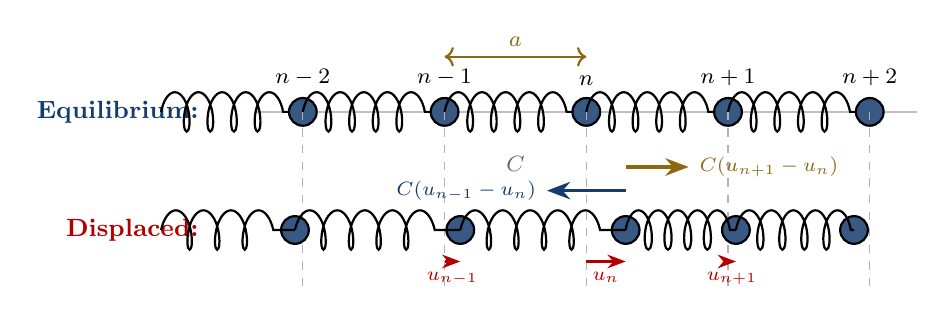
\begin{tikzpicture}[scale=1.0]
  % Equilibrium configuration
  \node[anchor=east,font=\small\bfseries,ntccblue] at (-0.6,1.5) {Equilibrium:};
  \draw[thick,gray!50] (0,1.5) -- (8.4,1.5);
  \foreach \x/\label in {0.6/{n-2}, 2.4/{n-1}, 4.2/{n}, 6.0/{n+1}, 7.8/{n+2}} {
    \draw[thick,decoration={coil,aspect=0.4,segment length=3mm,amplitude=2.5mm},decorate] (\x-1.8,1.5) -- (\x,1.5);
    \filldraw[fill=ntccblue!85,draw=black,thick] (\x,1.5) circle (5pt);
    \node[above=6pt,font=\footnotesize] at (\x,1.5) {$\label$};
    \draw[dashed,gray!60] (\x,1.5) -- (\x,-0.8);
  }
  % Spring constant label & lattice spacing
  \draw[<->,thick,ntccgold!80!black] (2.4,2.2) -- (4.2,2.2) node[midway,above,font=\footnotesize] {$a$};
  \node[below=4pt,font=\footnotesize,gray!80!black] at (3.3,1.2) {$C$};

  % Displaced configuration
  \node[anchor=east,font=\small\bfseries,red!70!black] at (-0.6,0.0) {Displaced:};
  % n-2 displaced by -0.1
  \filldraw[fill=ntccblue!85,draw=black,thick] (0.5,0.0) circle (5pt);
  % n-1 displaced by 0.2
  \filldraw[fill=ntccblue!85,draw=black,thick] (2.6,0.0) circle (5pt);
  % n displaced by 0.5
  \filldraw[fill=ntccblue!85,draw=black,thick] (4.7,0.0) circle (5pt);
  % n+1 displaced by 0.1
  \filldraw[fill=ntccblue!85,draw=black,thick] (6.1,0.0) circle (5pt);
  % n+2 displaced by -0.2
  \filldraw[fill=ntccblue!85,draw=black,thick] (7.6,0.0) circle (5pt);

  % Connecting springs in displaced state
  \draw[thick,decoration={coil,aspect=0.4,segment length=3.5mm,amplitude=2.5mm},decorate] (-1.2,0) -- (0.5,0);
  \draw[thick,decoration={coil,aspect=0.4,segment length=3.5mm,amplitude=2.5mm},decorate] (0.5,0) -- (2.6,0);
  \draw[thick,decoration={coil,aspect=0.4,segment length=3.5mm,amplitude=2.5mm},decorate] (2.6,0) -- (4.7,0);
  \draw[thick,decoration={coil,aspect=0.4,segment length=2.5mm,amplitude=2.5mm},decorate] (4.7,0) -- (6.1,0);
  \draw[thick,decoration={coil,aspect=0.4,segment length=2.8mm,amplitude=2.5mm},decorate] (6.1,0) -- (7.6,0);

  % Displacement arrows
  \draw[->,>=Stealth,thick,red!70!black] (2.4,-0.4) -- (2.6,-0.4) node[midway,below,font=\scriptsize] {$u_{n-1}$};
  \draw[->,>=Stealth,thick,red!70!black] (4.2,-0.4) -- (4.7,-0.4) node[midway,below,font=\scriptsize] {$u_n$};
  \draw[->,>=Stealth,thick,red!70!black] (6.0,-0.4) -- (6.1,-0.4) node[midway,below,font=\scriptsize] {$u_{n+1}$};

  % Net force arrows on atom n
  \draw[->,>=Stealth,very thick,ntccblue] (4.7,0.5) -- (3.7,0.5) node[left,font=\scriptsize] {$C(u_{n-1}-u_n)$};
  \draw[->,>=Stealth,very thick,ntccgold!80!black] (4.7,0.8) -- (5.5,0.8) node[right,font=\scriptsize] {$C(u_{n+1}-u_n)$};
\end{tikzpicture}
\caption{One-dimensional monoatomic harmonic chain. (Top) Equilibrium positions with lattice constant $a$. (Bottom) Dynamic state showing instantaneous atomic displacements $u_n$ and net restoring forces exerted by adjacent nearest-neighbour springs of force constant $C$.}
\label{fig:monoatomic_chain_model}
\end{figure}

\subsection{Monoatomic Linear Chain \hfill \small(20 min)}

\textbf{Setup.}
\begin{itemize}
\item Atoms of mass $M$ arranged in a 1D lattice with spacing $a$
\item Displacement of the $n$-th atom: $u_n$
\item Only nearest-neighbour springs, force constant $C$
\end{itemize}

\textbf{Equation of motion.}
\[
M\frac{d^2u_n}{dt^2} = C(u_{n+1}-u_n) - C(u_n-u_{n-1})
= C(u_{n+1}+u_{n-1}-2u_n)
\]

\textbf{Trial solution (plane wave).}
\[
u_n = A\,e^{i(kna-\omega t)}
\]
where $k$ is the wavevector and $\omega$ the angular frequency.

\textbf{Substitution.}
\[
-M\omega^2 = C\left(e^{ika}+e^{-ika}-2\right) = 2C(\cos ka - 1) = -4C\sin^2\!\left(\tfrac{ka}{2}\right)
\]

\begin{keybox}[Dispersion Relation]
\[
\omega(k) = 2\sqrt{\frac{C}{M}}\;\left|\sin\!\left(\frac{ka}{2}\right)\right|
\]
\end{keybox}

\textbf{Key features.}
\begin{enumerate}
\item \textbf{Periodic in $k$:} $\omega(k+2\pi/a)=\omega(k)$ $\Rightarrow$ only $k\in[-\pi/a,\pi/a]$ (first Brillouin zone) is physically distinct.
\item \textbf{Linear at small $k$:} $\omega \approx v_s|k|$, with $v_s = a\sqrt{C/M}$ the sound velocity.
\item \textbf{Maximum at zone boundary:} $\omega_{\max}=2\sqrt{C/M}$ at $k=\pm\pi/a$.
\item \textbf{Group velocity:} $v_g = d\omega/dk = a\sqrt{C/M}\,\cos(ka/2)$ $\to 0$ at the zone boundary.
\end{enumerate}

\begin{figure}[h]
\centering
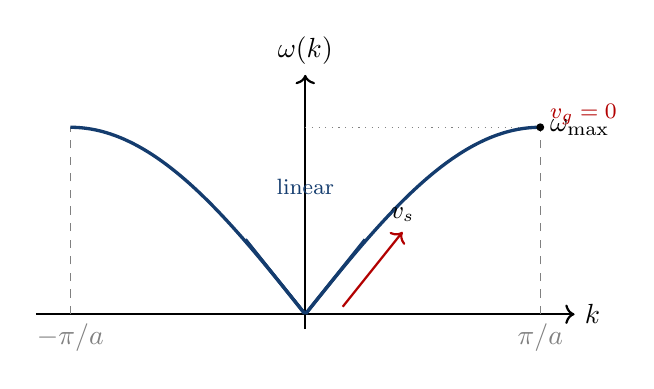
\begin{tikzpicture}[scale=0.95]
  % axes
  \draw[->,thick] (-3.6,0) -- (3.6,0) node[right] {$k$};
  \draw[->,thick] (0,-0.2) -- (0,3.2) node[above] {$\omega(k)$};
  % markers
  \draw[dashed,gray] (-3.1416,0) node[below] {$-\pi/a$} -- (-3.1416,2.5);
  \draw[dashed,gray] ( 3.1416,0) node[below] {$\pi/a$} -- ( 3.1416,2.5);
  \draw[dotted,gray] (0,2.5) -- (3.1416,2.5) node[right,black] {$\omega_{\max}$};
  % the dispersion: plot over [-pi, pi]
  \draw[ntccblue,very thick,domain=-3.1416:3.1416,samples=200]
    plot (\x, {2.5*abs(sin(deg(\x)/2))});
  % group velocity arrow near origin
  \draw[->,red!70!black,thick] (0.5,0.1) -- (1.3,1.1)
    node[above,black,font=\small] {$v_s$};
  % zone boundary annotation
  \fill (3.1416,2.5) circle (1.5pt);
  \node[above right,font=\footnotesize,red!70!black] at (3.1416,2.4) {$v_g=0$};
  % small-k region shading
  \begin{scope}
    \clip (-0.8,0) rectangle (0.8,3.2);
    \draw[ntccblue,very thick,domain=-0.8:0.8,samples=40]
      plot (\x, {1.25*abs(\x)});
  \end{scope}
  \node[font=\footnotesize,ntccblue] at (0,1.7) {linear};
\end{tikzpicture}
\caption{Dispersion $\omega(k)$ for the monoatomic chain. Linear (sound) near
$k=0$ with slope $v_s$; saturates at $\omega_{\max}=2\sqrt{C/M}$ at the zone
boundary $k=\pm\pi/a$, where the group velocity vanishes.}
\end{figure}

\begin{pitbox}[``Group velocity = 0'' does not mean the mode is a standing wave]
At the zone boundary, two counter-propagating plane waves of equal amplitude form a
standing wave, but a normal mode of the chain can be \emph{any} phase combination of
them. The vanishing of $v_g$ simply means that this particular mode does not
transport energy -- useful for thermal-resistance arguments later.
\end{pitbox}

\subsection{First Brillouin Zone \hfill \small(10 min)}

\textbf{Definition.} The first Brillouin zone is the Wigner--Seitz cell of the
reciprocal lattice. It contains all unique values of $k$ for which the dispersion
relation is not repeated.

\textbf{For the 1D chain:}
\begin{itemize}
\item Reciprocal lattice vector: $G = 2\pi/a$
\item First BZ: $k \in [-\pi/a,\pi/a]$
\end{itemize}

\textbf{Physical significance.}
\begin{itemize}
\item Modes with $k$ and $k+G$ are physically identical (same atomic displacements).
\item The number of allowed $k$-values in the first BZ equals the number of unit cells $N$.
\item With periodic boundary conditions: $k = \dfrac{2\pi n}{Na}$, $\ n=0,\pm1,\pm2,\dots,\pm N/2$.
\end{itemize}

\begin{physbox}[Recall from Module 1]
This is exactly the reciprocal-lattice / Wigner--Seitz construction you used for
X-ray diffraction, now applied to \emph{vibrational} wavevectors instead of
scattering wavevectors.
\end{physbox}

\begin{expbox}[How we measure this dispersion: inelastic neutron scattering]
Neutrons are the workhorse for phonon dispersion measurements because their
kinetic energy ($\sim$meV--eV) matches phonon energies, and they couple directly
to atomic nuclei (not to electron density). A monochromatic neutron beam of
wavevector $\mathbf k_i$ is scattered into $\mathbf k_f$, with energy loss
$\hbar\omega = \tfrac{\hbar^2}{2m_n}(k_i^2-k_f^2)$ and momentum transfer
$\mathbf Q = \mathbf k_f-\mathbf k_i$. Conservation modulo a reciprocal lattice
vector gives a phonon dispersion point $(\mathbf Q,\omega)$. Pioneered at
Brookhaven and Chalk River in the 1960s; standard textbook experiment.
\end{expbox}

\subsection{Density of States in 1D \hfill \small(7 min)}

\textbf{Definition.} The density of states $g(\omega)$ gives the number of modes per
unit frequency interval.

\textbf{For the 1D monoatomic chain:}
\[
g(\omega)\,d\omega = \frac{L}{\pi}\,dk = \frac{L}{\pi}\frac{dk}{d\omega}\,d\omega,
\qquad
g(\omega) = \frac{L}{\pi v_g} = \frac{L}{\pi a\sqrt{C/M}\,\cos(ka/2)}
\]
Using $\cos(ka/2)=\sqrt{1-\sin^2(ka/2)}=\sqrt{1-(\omega/\omega_{\max})^2}$:
\begin{keybox}[1D Density of States]
\[
g(\omega) = \frac{2L}{\pi\sqrt{\omega_{\max}^2-\omega^2}}
\]
\end{keybox}
This diverges at $\omega=\omega_{\max}$ -- a \textbf{Van Hove singularity}, arising
because $v_g\to0$ there (flat top of the dispersion curve).

\begin{figure}[h]
\centering
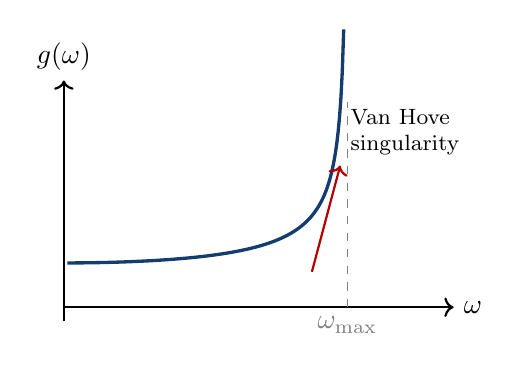
\begin{tikzpicture}[scale=0.9]
  % axes
  \draw[->,thick] (0,0) -- (5.5,0) node[right] {$\omega$};
  \draw[->,thick] (0,-0.2) -- (0,3.2) node[above] {$g(\omega)$};
  % markers
  \draw[dashed,gray] (4.0,0) node[below] {$\omega_{\max}$} -- (4.0,2.9);
  % the 1D DOS: g ~ 1/sqrt(wmax^2 - w^2)
  \draw[ntccblue,very thick,domain=0.05:3.95,samples=200]
    plot (\x, {2.5/sqrt(16-\x*\x)});
  % divergence marker
  \draw[->,red!70!black,thick] (3.5,0.5) -- (3.9,2.0)
    node[above right,align=left,font=\footnotesize,black] {Van Hove\\singularity};
\end{tikzpicture}
\caption{1D monoatomic chain density of states. The square-root divergence at
$\omega_{\max}$ is the simplest example of a Van Hove singularity, arising from
the vanishing group velocity at the zone boundary.}
\end{figure}

\begin{figure}[htbp]
\centering
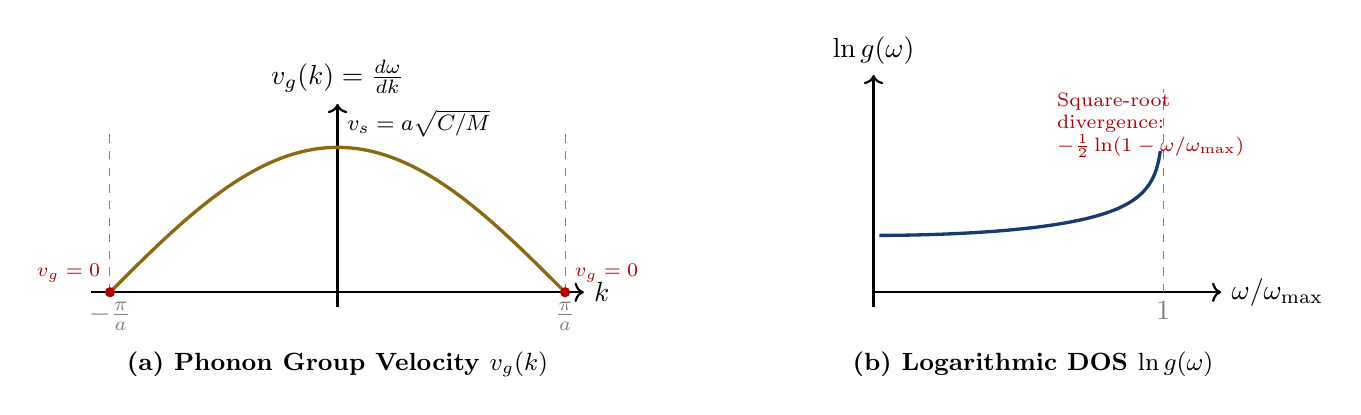
\begin{tikzpicture}[scale=0.92]
  % (a) Group velocity
  \begin{scope}[xshift=0cm]
    \draw[->,thick] (-3.4,0) -- (3.4,0) node[right] {$k$};
    \draw[->,thick] (0,-0.2) -- (0,2.6) node[above] {$v_g(k) = \frac{d\omega}{dk}$};
    \draw[dashed,gray] (-3.1416,0) node[below] {$-\frac{\pi}{a}$} -- (-3.1416,2.2);
    \draw[dashed,gray] (3.1416,0) node[below] {$\frac{\pi}{a}$} -- (3.1416,2.2);
    \draw[ntccgold!80!black,very thick,domain=-3.1416:3.1416,samples=150]
      plot (\x, {2.0*cos(deg(\x/2))});
    \node[above right,font=\footnotesize] at (0,2.0) {$v_s = a\sqrt{C/M}$};
    \fill[red!70!black] (-3.1416,0) circle (2pt) node[above left,font=\scriptsize] {$v_g=0$};
    \fill[red!70!black] (3.1416,0) circle (2pt) node[above right,font=\scriptsize] {$v_g=0$};
    \node[font=\bfseries\small] at (0,-1.0) {(a) Phonon Group Velocity $v_g(k)$};
  \end{scope}

  % (b) Log-scale DOS
  \begin{scope}[xshift=7.4cm]
    \draw[->,thick] (0,0) -- (4.8,0) node[right] {$\omega/\omega_{\max}$};
    \draw[->,thick] (0,-0.2) -- (0,3.0) node[above] {$\ln g(\omega)$};
    \draw[dashed,gray] (4.0,0) node[below] {$1$} -- (4.0,2.8);
    \draw[ntccblue,very thick,domain=0.08:3.96,samples=180]
      plot (\x, {0.6*ln(2.0/sqrt(16.0 - \x*\x)) + 1.2});
    \node[right,font=\scriptsize,red!70!black,align=left] at (2.4,2.3) {Square-root\\divergence:\\$-\frac{1}{2}\ln(1-\omega/\omega_{\max})$};
    \node[font=\bfseries\small] at (2.2,-1.0) {(b) Logarithmic DOS $\ln g(\omega)$};
  \end{scope}
\end{tikzpicture}
\caption{(a) Phonon group velocity $v_g(k) = v_s \cos(ka/2)$, demonstrating the acoustic limit ($v_g = v_s$ at $k=0$) and zero velocity at the Brillouin zone edge. (b) 1D density of states on a logarithmic scale, highlighting the integrable Van Hove singularity at $\omega = \omega_{\max}$.}
\label{fig:group_vel_and_log_dos}
\end{figure}

\subsection{Computational Illustration \hfill \small(5 min)}

The dispersion relation and group velocity of the monoatomic chain can be visualised
directly from the closed-form expressions derived above:
\[
\omega(k)=2\sqrt{C/M}\,|\sin(ka/2)|, \qquad v_g(k)=a\sqrt{C/M}\,\cos(ka/2).
\]
Plotting both across the first Brillouin zone $k\in[-\pi/a,\pi/a]$ makes the
zero-group-velocity condition at the zone boundary especially clear -- this is a good
in-class or take-home numerical exercise (e.g.\ using NumPy/Matplotlib).

\begin{pybox}[Python: dispersion and group velocity of a monoatomic chain]
\begin{lstlisting}
import numpy as np
import matplotlib.pyplot as plt

# --- Parameters (SI) ---
M = 1.66e-27 * 40      # 40 amu -> kg
C = 50.0               # N/m
a = 3.0e-10            # m

# Derived quantities
omega_max = 2.0*np.sqrt(C/M)         # rad/s
v_s       = a*np.sqrt(C/M)           # sound velocity, m/s

# Wavevector sweep across the first Brillouin zone
k = np.linspace(-np.pi/a, np.pi/a, 1001)
omega = omega_max * np.abs(np.sin(k*a/2.0))
v_g   = a*np.sqrt(C/M) * np.cos(k*a/2.0)

fig, (ax1, ax2) = plt.subplots(1, 2, figsize=(9, 3.5))

ax1.plot(k*a, omega)
ax1.set_xlabel(r'$ka$')
ax1.set_ylabel(r'$\omega(k)$ (rad/s)')
ax1.set_title('Dispersion')
ax1.axvline(np.pi, color='gray', ls=':')
ax1.text(np.pi, omega_max*0.95, r'$\pi$', ha='center')

ax2.plot(k*a, v_g)
ax2.set_xlabel(r'$ka$')
ax2.set_ylabel(r'$v_g(k)$ (m/s)')
ax2.set_title('Group velocity')
ax2.axhline(0, color='k', lw=0.5)
ax2.axvline(np.pi, color='gray', ls=':')

plt.tight_layout()
plt.show()

# Sanity check: print the speed of sound
print(f"v_s = {v_s:.3e} m/s,  omega_max = {omega_max:.3e} rad/s")
\end{lstlisting}
\end{pybox}

\begin{takebox}[Take-home message of Lecture 8]
A 1D monatomic chain has $N$ modes in the first BZ, with dispersion
$\omega(k)=2\sqrt{C/M}\,|\sin(ka/2)|$. The mode is acoustic: $\omega\to0$ as $k\to0$.
The 1D DOS diverges as $1/\sqrt{\omega_{\max}^2-\omega^2}$ at the zone edge.
\end{takebox}

\begin{probbox}
\begin{enumerate}
\item Show that the sound velocity in a monoatomic chain is $v_s=a\sqrt{C/M}$.
\item Calculate the density of states at $\omega=\omega_{\max}/2$ for a chain of 1000 atoms.
\item What happens to the group velocity at the zone boundary? Explain physically.
\end{enumerate}
\end{probbox}

\newpage
% ======================================================================
\lecheader{9}{Diatomic Linear Chain and Optical Phonons}{50 minutes}

\begin{keybox}[Learning Objectives]
\begin{itemize}
\item Derive the dispersion relation for a diatomic chain
\item Distinguish acoustic and optical branches
\item Understand the physical nature of optical modes
\end{itemize}
\end{keybox}

\begin{histbox}[Why the diatomic chain is worth knowing]
The diatomic chain is the simplest model that exhibits the two essential features
of any crystal with more than one atom per unit cell: two branches (acoustic,
optical) and a \emph{forbidden frequency gap} at the zone boundary. The same
physics controls the existence of electronic band gaps in semiconductors -- the
mathematical structure (a $2\times2$ secular equation) is identical, with
``mass'' replaced by ``on-site energy'' and ``spring constant'' replaced by
``hopping amplitude.''
\end{histbox}

\subsection{Setup and Equations of Motion \hfill \small(12 min)}

\textbf{Setup.}
\begin{itemize}
\item Two types of atoms, masses $M$ and $m$ ($M>m$)
\item Alternating arrangement with spacing $a/2$ between neighbours
\item Lattice constant $a$ (repeat distance)
\item Same force constant $C$ for all nearest-neighbour bonds
\end{itemize}

\begin{figure}[htbp]
\centering
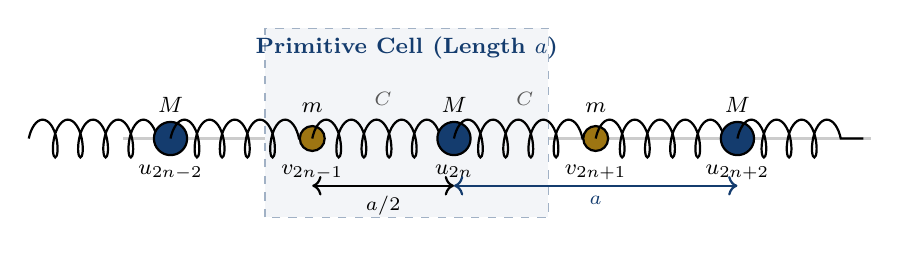
\begin{tikzpicture}[scale=1.0]
  % Backbone
  \draw[thick,gray!40] (0,0) -- (9.5,0);
  % Unit cell box
  \draw[dashed,fill=ntccblue!5,draw=ntccblue!40] (1.8,-1.0) rectangle (5.4,1.4);
  \node[font=\footnotesize\bfseries,ntccblue] at (3.6,1.15) {Primitive Cell (Length $a$)};

  % Atoms
  \foreach \x/\m/\label/\col/\sz in {
    0.6/M/{u_{2n-2}}/ntccblue/6pt,
    2.4/m/{v_{2n-1}}/ntccgold!90!black/4.5pt,
    4.2/M/{u_{2n}}/ntccblue/6pt,
    6.0/m/{v_{2n+1}}/ntccgold!90!black/4.5pt,
    7.8/M/{u_{2n+2}}/ntccblue/6pt
  } {
    \draw[thick,decoration={coil,aspect=0.4,segment length=3.2mm,amplitude=2.4mm},decorate] (\x-1.8,0) -- (\x,0);
    \filldraw[fill=\col,draw=black,thick] (\x,0) circle (\sz);
    \node[below=6pt,font=\footnotesize] at (\x,0) {$\label$};
    \node[above=6pt,font=\footnotesize\bfseries] at (\x,0) {$\m$};
  }
  % Spring to right
  \draw[thick,decoration={coil,aspect=0.4,segment length=3.2mm,amplitude=2.4mm},decorate] (7.8,0) -- (9.4,0);

  % Spacings
  \draw[<->,thick] (2.4,-0.6) -- (4.2,-0.6) node[midway,below,font=\scriptsize] {$a/2$};
  \draw[<->,thick,ntccblue] (4.2,-0.6) -- (7.8,-0.6) node[midway,below,font=\scriptsize] {$a$};
  \node[above,font=\scriptsize,gray!70!black] at (3.3,0.3) {$C$};
  \node[above,font=\scriptsize,gray!70!black] at (5.1,0.3) {$C$};
\end{tikzpicture}
\caption{One-dimensional diatomic lattice chain with alternating masses $M > m$ and identical spring constants $C$. The primitive unit cell has length $a$ and contains two basis atoms with equilibrium spacing $a/2$.}
\label{fig:diatomic_chain_schematic}
\end{figure}

\textbf{Equations of motion.}\\
Even sites (mass $M$):
\[
M\frac{d^2u_{2n}}{dt^2} = C(v_{2n+1}+v_{2n-1}-2u_{2n})
\]
Odd sites (mass $m$):
\[
m\frac{d^2v_{2n+1}}{dt^2} = C(u_{2n+2}+u_{2n}-2v_{2n+1})
\]

\textbf{Trial solutions.}
\[
u_{2n} = A\,e^{i(nka-\omega t)}, \qquad
v_{2n+1} = B\,e^{i(nka+ka/2-\omega t)}
\]

\subsection{Dispersion Relation Derivation \hfill \small(18 min)}

Substituting the trial solutions:
\[
-M\omega^2A = C\!\left(2B\cos\tfrac{ka}{2}-2A\right),\qquad
-m\omega^2B = C\!\left(2A\cos\tfrac{ka}{2}-2B\right)
\]
Rearranged into matrix form:
\[
(2C-M\omega^2)A - 2C\cos\!\left(\tfrac{ka}{2}\right)B = 0, \qquad
-2C\cos\!\left(\tfrac{ka}{2}\right)A + (2C-m\omega^2)B = 0
\]

\textbf{Secular equation} (determinant $=0$):
\[
\begin{vmatrix} 2C-M\omega^2 & -2C\cos(ka/2)\\[2pt] -2C\cos(ka/2) & 2C-m\omega^2\end{vmatrix}=0
\]
\[
(2C-M\omega^2)(2C-m\omega^2) - 4C^2\cos^2\!\left(\tfrac{ka}{2}\right)=0
\]

\textbf{Expanded (filled-in step).} Let $x\equiv\omega^2$. Multiplying out:
\[
4C^2 - 2C(M+m)x + Mm x^2 - 4C^2\cos^2\!\left(\tfrac{ka}{2}\right) = 0.
\]
Using $\cos^2(\theta)=\tfrac12(1+\cos 2\theta)$ and $1-\cos 2\theta = 2\sin^2\theta$:
\[
4C^2\bigl[1-\cos^2(\tfrac{ka}{2})\bigr] = 4C^2\sin^2(\tfrac{ka}{2}),
\]
so the secular equation simplifies to
\begin{keybox}[Quadratic in $\omega^2$]
\[
Mm\,\omega^4 - 2C(M+m)\,\omega^2 + 4C^2\sin^2\!\left(\tfrac{ka}{2}\right)=0
\]
\end{keybox}

The quadratic formula in $\omega^2$ gives
\begin{keybox}[Dispersion Relation -- Two Branches]
\[
\omega_\pm^2 = C\left(\frac1M+\frac1m\right) \pm C\sqrt{\left(\frac1M+\frac1m\right)^2 - \frac{4\sin^2(ka/2)}{Mm}}
\]
\end{keybox}

\begin{figure}[htbp]
\centering
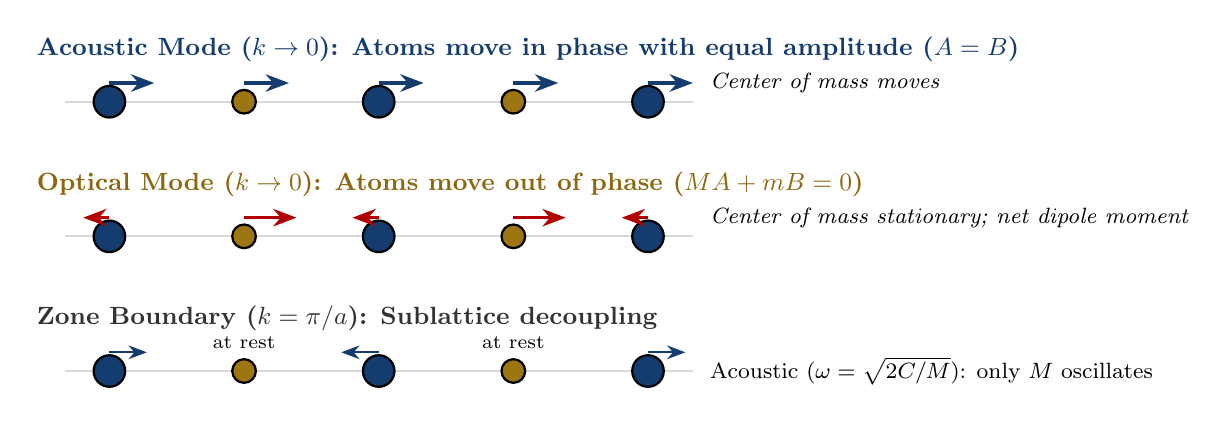
\begin{tikzpicture}[scale=0.95]
  % (a) Acoustic mode at k -> 0
  \begin{scope}[yshift=2.6cm]
    \node[anchor=west,font=\small\bfseries,ntccblue] at (-0.5,0.7) {Acoustic Mode ($k \to 0$): Atoms move in phase with equal amplitude ($A = B$)};
    \draw[thick,gray!30] (0,0) -- (8.4,0);
    \foreach \x/\m/\sz/\col in {0.6/M/6pt/ntccblue, 2.4/m/4.5pt/ntccgold!90!black, 4.2/M/6pt/ntccblue, 6.0/m/4.5pt/ntccgold!90!black, 7.8/M/6pt/ntccblue} {
      \filldraw[fill=\col,draw=black,thick] (\x,0) circle (\sz);
      \draw[->,>=Stealth,very thick,ntccblue] (\x,0.25) -- (\x+0.6,0.25);
    }
    \node[right,font=\footnotesize\itshape] at (8.5,0.25) {Center of mass moves};
  \end{scope}

  % (b) Optical mode at k -> 0
  \begin{scope}[yshift=0.8cm]
    \node[anchor=west,font=\small\bfseries,ntccgold!80!black] at (-0.5,0.7) {Optical Mode ($k \to 0$): Atoms move out of phase ($MA + mB = 0$)};
    \draw[thick,gray!30] (0,0) -- (8.4,0);
    \foreach \x/\m/\sz/\col/\dir in {0.6/M/6pt/ntccblue/-0.35, 2.4/m/4.5pt/ntccgold!90!black/0.7, 4.2/M/6pt/ntccblue/-0.35, 6.0/m/4.5pt/ntccgold!90!black/0.7, 7.8/M/6pt/ntccblue/-0.35} {
      \filldraw[fill=\col,draw=black,thick] (\x,0) circle (\sz);
      \draw[->,>=Stealth,very thick,red!70!black] (\x,0.25) -- (\x+\dir,0.25);
    }
    \node[right,font=\footnotesize\itshape] at (8.5,0.25) {Center of mass stationary; net dipole moment};
  \end{scope}

  % (c) Zone boundary k = pi/a
  \begin{scope}[yshift=-1.0cm]
    \node[anchor=west,font=\small\bfseries,black!80] at (-0.5,0.7) {Zone Boundary ($k = \pi/a$): Sublattice decoupling};
    \draw[thick,gray!30] (0,0) -- (8.4,0);
    % Acoustic: only heavy atoms move
    \filldraw[fill=ntccblue,draw=black,thick] (0.6,0) circle (6pt); \draw[->,>=Stealth,thick,ntccblue] (0.6,0.25) -- (1.1,0.25);
    \filldraw[fill=ntccgold!90!black,draw=black,thick] (2.4,0) circle (4.5pt); \node[above=2pt,font=\scriptsize] at (2.4,0.1) {at rest};
    \filldraw[fill=ntccblue,draw=black,thick] (4.2,0) circle (6pt); \draw[->,>=Stealth,thick,ntccblue] (4.2,0.25) -- (3.7,0.25);
    \filldraw[fill=ntccgold!90!black,draw=black,thick] (6.0,0) circle (4.5pt); \node[above=2pt,font=\scriptsize] at (6.0,0.1) {at rest};
    \filldraw[fill=ntccblue,draw=black,thick] (7.8,0) circle (6pt); \draw[->,>=Stealth,thick,ntccblue] (7.8,0.25) -- (8.3,0.25);
    \node[right,font=\footnotesize] at (8.5,0) {Acoustic ($\omega = \sqrt{2C/M}$): only $M$ oscillates};
  \end{scope}
\end{tikzpicture}
\caption{Physical displacement configurations of the diatomic chain. In the acoustic branch at $k \to 0$, basis atoms move together in phase. In the optical branch at $k \to 0$, opposite charges oscillate against each other, producing an oscillating electric dipole moment. At the zone boundary $k = \pi/a$, the two sublattices decouple completely.}
\label{fig:diatomic_mode_patterns}
\end{figure}

\subsection{Analysis of Branches \hfill \small(12 min)}

\textbf{Acoustic branch $(\omega_-)$.}
\begin{itemize}
\item At $k=0$: $\omega_-=0$, $A=B$ (atoms move in phase).
\item At $k=\pi/a$: $\omega_-=\sqrt{2C/M}$ (for $M>m$); $A/B=0$ (heavy atoms move, light atoms stationary).
\item Linear at small $k$: $\omega_- \approx v_s|k|$, $v_s = a\sqrt{C/(2(M+m))}$.
\item Called ``acoustic'' because at long wavelength these are ordinary sound waves.
\end{itemize}

\textbf{Optical branch $(\omega_+)$.}
\begin{itemize}
\item At $k=0$: $\omega_+=\sqrt{2C(1/M+1/m)}$, $A/B=-m/M$ (atoms move out of phase).
\item At $k=\pi/a$: $\omega_+=\sqrt{2C/m}$, $B=0$ (light atoms move, heavy atoms stationary).
\item Called ``optical'' because in ionic crystals these modes couple to infrared light
(the oscillating electric field drives oppositely-charged ions in opposite directions).
\end{itemize}

\begin{keybox}[Key observation]
There is a \textbf{frequency gap} between $\sqrt{2C/M}$ and $\sqrt{2C/m}$ at
$k=\pi/a$. No propagating modes exist in this gap.
\end{keybox}

\begin{figure}[h]
\centering
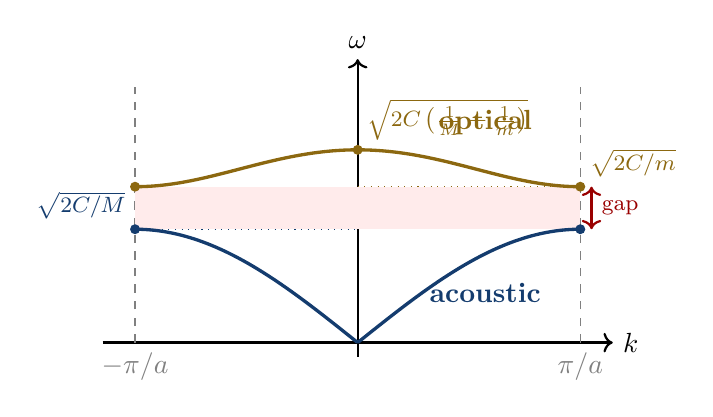
\begin{tikzpicture}[scale=0.9]
  % axes
  \draw[->,thick] (-3.6,0) -- (3.6,0) node[right] {$k$};
  \draw[->,thick] (0,-0.2) -- (0,4.0) node[above] {$\omega$};
  \draw[dashed,gray] (-3.1416,0) node[below] {$-\pi/a$} -- (-3.1416,3.6);
  \draw[dashed,gray] ( 3.1416,0) node[below] {$\pi/a$}  -- ( 3.1416,3.6);

  % gap region
  \begin{scope}
    \fill[red!8] (-3.1416,1.6) rectangle (3.1416,2.2);
    \draw[<->,red!60!black,thick] (3.3,1.6) -- (3.3,2.2)
      node[midway,right,font=\footnotesize] {gap};
  \end{scope}

  % acoustic branch (bottom)
  \draw[ntccblue,very thick,domain=-3.1416:3.1416,samples=200]
    plot (\x, {1.6*sin(deg(0.5*abs(\x)))});

  % optical branch (top)
  \draw[ntccgold!80!black,very thick,domain=-3.1416:3.1416,samples=200]
    plot (\x, {sqrt(2.2*2.2 + 1.6*1.6 - 1.6*1.6*sin(deg(0.5*abs(\x)))*sin(deg(0.5*abs(\x))))});

  % labels
  \node[ntccblue,font=\bfseries] at (1.8,0.7) {acoustic};
  \node[ntccgold!80!black,font=\bfseries] at (1.8,3.1) {optical};

  % branch boundary points and values
  \fill[ntccblue] (-3.1416,1.6) circle (2pt);
  \fill[ntccblue] (3.1416,1.6) circle (2pt);
  \node[above left,font=\footnotesize,ntccblue] at (-3.1416,1.6) {$\sqrt{2C/M}$};
  \draw[dotted,ntccblue] (-3.1416,1.6) -- (0,1.6);

  \fill[ntccgold!80!black] (-3.1416,2.2) circle (2pt);
  \fill[ntccgold!80!black] (3.1416,2.2) circle (2pt);
  \node[above right,font=\footnotesize,ntccgold!80!black] at (3.1416,2.2) {$\sqrt{2C/m}$};
  \draw[dotted,ntccgold!80!black] (0,2.2) -- (3.1416,2.2);

  \fill[ntccgold!80!black] (0,2.72) circle (2pt);
  \node[above right,font=\footnotesize,ntccgold!80!black] at (0,2.72) {$\sqrt{2C\left(\frac{1}{M}+\frac{1}{m}\right)}$};
\end{tikzpicture}
\caption{Schematic diatomic-chain dispersion. The shaded band between
$\sqrt{2C/M}$ and $\sqrt{2C/m}$ is the forbidden frequency gap. Real systems
have this gap renormalised by the actual force-constant tensor, but the topology
is generic.}
\end{figure}

\subsection{Physical Interpretation \hfill \small(5 min)}

\begin{physbox}[Acoustic mode, $k\approx0$]
Both sublattices move together -- a macroscopic elastic deformation.
\end{physbox}
\begin{physbox}[Optical mode, $k\approx0$]
Sublattices move against each other -- no centre-of-mass motion, but internal
strain. In polar crystals this creates an oscillating dipole moment that couples to
electromagnetic radiation.
\end{physbox}
\begin{physbox}[Zone boundary, $k=\pi/a$]
One sublattice is stationary while the other vibrates; which one depends on the
branch.
\end{physbox}

\begin{expbox}[Direct observation: Raman and infrared spectroscopy]
The $k=0$ optical mode is the one that couples to light. In a polar (ionic)
crystal like NaCl or GaAs, this mode is \emph{infrared active} -- a long-wavelength
EM wave drives the two oppositely-charged sublattices against each other. In
non-polar crystals (Si, Ge, diamond) the $k=0$ optical mode can be \emph{Raman
active}: the oscillating strain modulates the electronic polarisability, scattering
light inelastically with a frequency shift equal to the optical phonon frequency.
Raman and IR are thus complementary, and the LO--TO splitting (Lec 14) controls
which modes are seen in which experiment.
\end{expbox}

\subsection{Computational Illustration \hfill \small(3 min)}

\begin{pybox}[Python: plot the two branches of the diatomic chain]
\begin{lstlisting}
import numpy as np
import matplotlib.pyplot as plt

# Parameters (arbitrary units: M=2, m=1, C=1, a=1)
M, m, C, a = 2.0, 1.0, 1.0, 1.0

k = np.linspace(-np.pi/a, np.pi/a, 1001)
s = np.sin(k*a/2.0)

# Closed-form omega_+^2 and omega_-^2
inv = (1.0/M + 1.0/m)
disc = np.sqrt(inv**2 - 4.0*s**2/(M*m))
omega_p = np.sqrt(C*(inv + disc))
omega_m = np.sqrt(C*(inv - disc))

# Sanity checks
print(f"omega_- at k=0      = {omega_m[500]:.4f}  (should be 0)")
print(f"omega_- at k=pi/a   = {omega_m[-1]:.4f}  (should be sqrt(2C/M) = {np.sqrt(2*C/M):.4f})")
print(f"omega_+ at k=0      = {omega_p[500]:.4f}  (should be sqrt(2C/M+2C/m) = {np.sqrt(2*C*(1/M+1/m)):.4f})")
print(f"omega_+ at k=pi/a   = {omega_p[-1]:.4f}  (should be sqrt(2C/m) = {np.sqrt(2*C/m):.4f})")

fig, ax = plt.subplots(figsize=(6, 4))
ax.plot(k*a, omega_p, color='tab:orange', label=r'optical $\omega_+$')
ax.plot(k*a, omega_m, color='tab:blue',   label=r'acoustic $\omega_-$')
ax.set_xlabel(r'$ka$')
ax.set_ylabel(r'$\omega_\pm(k)$')
ax.axvspan(0, np.pi, color='red', alpha=0.06)
ax.legend()
plt.tight_layout()
plt.show()
\end{lstlisting}
\end{pybox}

\begin{pitbox}[``Acoustic'' and ``optical'' names are not about which atoms move]
The naming refers to \emph{what the mode couples to}, not who is moving. Acoustic
modes are the ones that, at long wavelength, are sound -- they couple to macroscopic
strain. Optical modes couple to electromagnetic radiation (in polar materials).
A heavy atom moving alone at the zone boundary is still an acoustic mode if the
dispersion branch is the lower one; the labels are fixed by the branch, not the
instantaneous displacement pattern.
\end{pitbox}

\begin{probbox}
\begin{enumerate}
\item Show that for $M=m$ the diatomic chain reduces to the monoatomic case with
lattice constant $a/2$.
\item Calculate the frequency gap for a diatomic chain with $M=40$ amu, $m=20$ amu,
$C=50$~N/m.
\item Explain why the optical branch is flat near $k=0$ in real 3D crystals.
\end{enumerate}
\end{probbox}

\newpage
% ======================================================================
\lecheader{10}{Phonons -- Quantization of Lattice Vibrations}{50 minutes}

\begin{keybox}[Learning Objectives]
\begin{itemize}
\item Understand phonons as quantum quasiparticles
\item Derive phonon energy and momentum
\item Apply Bose--Einstein statistics to phonons
\end{itemize}
\end{keybox}

\begin{histbox}[Phonons: a 20th-century name for an old idea]
The word ``phonon'' was coined by Yakov Frenkel in 1932, drawing an explicit
analogy with the photon. The underlying physics is just the second-quantised
harmonic oscillator: any normal mode of the lattice, treated quantum mechanically,
is a bosonic field with energy quanta $\hbar\omega$. The Bose--Einstein distribution
that we will use was developed by Bose (1924) and Einstein (1924--25) for photons;
its application to phonons is a one-line replacement of the dispersion.
\end{histbox}

\subsection{Classical to Quantum: Normal Modes \hfill \small(12 min)}

\textbf{Classical picture.} A crystal with $N$ atoms has $3N$ degrees of freedom. In
the harmonic approximation the Hamiltonian diagonalises into $3N$ independent
harmonic oscillators (normal modes).

\textbf{Quantum picture.} Each normal mode of frequency $\omega$ is quantised like a
harmonic oscillator:
\[
E_n = \left(n+\frac12\right)\hbar\omega, \qquad n=0,1,2,\dots
\]

\begin{keybox}[Definition -- Phonon]
A phonon is the quantum of lattice vibrational energy. It is a \textbf{quasiparticle}
with
\begin{itemize}
\item Energy $E=\hbar\omega$
\item (Crystal) momentum $\mathbf p = \hbar\mathbf k$
\item Spin $0$ (boson)
\end{itemize}
\end{keybox}

\begin{physbox}[Important distinction]
Phonons are \emph{not} real particles carrying physical momentum. $\hbar\mathbf k$
is \emph{crystal momentum} -- conserved only modulo a reciprocal lattice vector.
Phonons are collective excitations of the entire lattice.
\end{physbox}

\subsection{Phonon Creation and Annihilation \hfill \small(15 min)}

\textbf{Ladder operators.} For each mode $(\mathbf k,s)$, $s$ labelling polarisation:
\[
a^\dagger_{\mathbf k s}\ket{n_{\mathbf k s}} = \sqrt{n_{\mathbf k s}+1}\,\ket{n_{\mathbf k s}+1},
\qquad
a_{\mathbf k s}\ket{n_{\mathbf k s}} = \sqrt{n_{\mathbf k s}}\,\ket{n_{\mathbf k s}-1}
\]

\textbf{Hamiltonian.}
\[
H = \sum_{\mathbf k,s}\hbar\omega_{\mathbf k s}\left(a^\dagger_{\mathbf k s}a_{\mathbf k s}+\frac12\right)
\]

\textbf{Number operator.} $n_{\mathbf k s}=a^\dagger_{\mathbf k s}a_{\mathbf k s}$
gives the number of phonons in mode $(\mathbf k,s)$.

\begin{figure}[htbp]
\centering
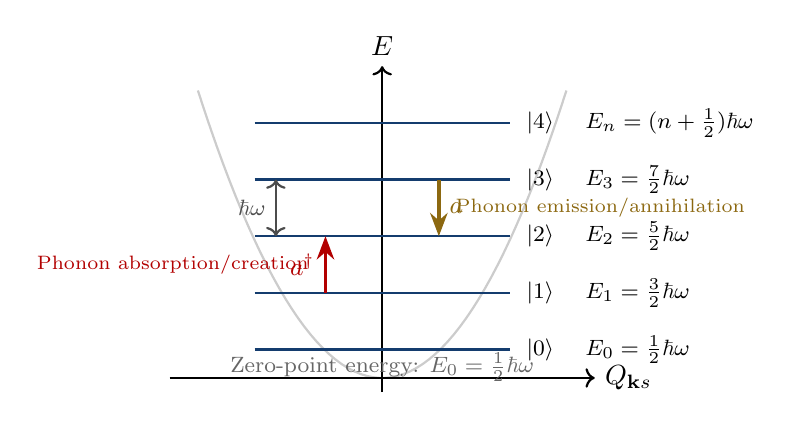
\begin{tikzpicture}[scale=0.9]
  % Potential well parabola
  \draw[thick,gray!40,domain=-2.6:2.6,samples=60] plot (\x, {0.6*\x*\x});
  \draw[->,thick] (-3.0,0) -- (3.0,0) node[right] {$Q_{\mathbf{k}s}$};
  \draw[->,thick] (0,-0.2) -- (0,4.4) node[above] {$E$};

  % Energy levels
  \foreach \n/\y/\lab in {0/0.4/{E_0 = \frac{1}{2}\hbar\omega}, 1/1.2/{E_1 = \frac{3}{2}\hbar\omega}, 2/2.0/{E_2 = \frac{5}{2}\hbar\omega}, 3/2.8/{E_3 = \frac{7}{2}\hbar\omega}, 4/3.6/{E_n = (n+\frac{1}{2})\hbar\omega}} {
    \draw[thick,ntccblue] (-1.8,\y) -- (1.8,\y);
    \node[right,font=\footnotesize] at (1.9,\y) {$\ket{\n}$ \quad $\lab$};
  }

  % Ladder operator arrows
  \draw[->,>=Stealth,very thick,red!70!black] (-0.8,1.2) -- (-0.8,2.0) node[midway,left,font=\small] {$a^\dagger$};
  \node[left,font=\scriptsize,red!70!black] at (-0.9,1.6) {Phonon absorption/creation};

  \draw[->,>=Stealth,very thick,ntccgold!80!black] (0.8,2.8) -- (0.8,2.0) node[midway,right,font=\small] {$a$};
  \node[right,font=\scriptsize,ntccgold!80!black] at (0.9,2.4) {Phonon emission/annihilation};

  % Spacing marker
  \draw[<->,thick,black!70] (-1.5,2.0) -- (-1.5,2.8) node[midway,left,font=\footnotesize] {$\hbar\omega$};
  \node[font=\footnotesize,gray!80!black] at (0,0.15) {Zero-point energy: $E_0 = \frac{1}{2}\hbar\omega$};
\end{tikzpicture}
\caption{Harmonic oscillator energy ladder for a single normal mode $(\mathbf{k}, s)$. The creation operator $a^\dagger$ adds a phonon of energy $\hbar\omega$, while the annihilation operator $a$ removes one. The vacuum ground state has persistent zero-point energy $\frac{1}{2}\hbar\omega$.}
\label{fig:phonon_ladder_diagram}
\end{figure}

\begin{physbox}[Physical interpretation]
\begin{itemize}
\item $a^\dagger_{\mathbf k s}$ creates a phonon; $a_{\mathbf k s}$ annihilates one.
\item The ground state ($T=0$) has \textbf{zero-point energy} $\sum \hbar\omega/2$.
\end{itemize}
\end{physbox}

\begin{pitbox}[``Crystal momentum is conserved modulo $\mathbf G$'']
This is the single most-violated rule in solid-state homework. When two phonons
collide, $\mathbf k_1+\mathbf k_2$ need not equal $\mathbf k_3$; it only has to
equal $\mathbf k_3$ plus \emph{some} reciprocal lattice vector. The cases $\mathbf G=0$
and $\mathbf G\ne0$ are called \emph{normal} and \emph{Umklapp} processes,
respectively. The latter are essential for thermal resistance (Lec 13) and for
electrical resistivity at high $T$.
\end{pitbox}

\subsection{Bose--Einstein Statistics \hfill \small(12 min)}

Phonons are bosons (integer spin, no Pauli exclusion). The average occupation number
of a phonon mode at temperature $T$ is the \textbf{Planck} (Bose--Einstein)
distribution:
\begin{keybox}[Bose--Einstein Occupation]
\[
\langle n_{\mathbf k s}\rangle = \frac{1}{e^{\hbar\omega_{\mathbf ks}/k_BT}-1} = n_B(\omega_{\mathbf k s})
\]
\end{keybox}

\textbf{Limiting cases.}
\begin{itemize}
\item High $T$ ($k_BT\gg\hbar\omega$): $n_B\approx k_BT/\hbar\omega \gg 1$ (classical equipartition).
\item Low $T$ ($k_BT\ll\hbar\omega$): $n_B\approx e^{-\hbar\omega/k_BT}\ll 1$ (quantum regime).
\end{itemize}

\textbf{Total energy.}
\[
U = \sum_{\mathbf k,s}\hbar\omega_{\mathbf k s}\left(\langle n_{\mathbf ks}\rangle+\frac12\right)
\]

\subsection{Crystal Momentum Conservation \hfill \small(8 min)}

\textbf{Umklapp processes.} In phonon--phonon or phonon--electron interactions,
crystal momentum is conserved \emph{modulo} a reciprocal lattice vector:
\[
\mathbf k_1+\mathbf k_2 = \mathbf k_3+\mathbf G
\]
\begin{itemize}
\item $\mathbf G=0$: \textbf{Normal process} -- total crystal momentum conserved.
\item $\mathbf G\ne0$: \textbf{Umklapp process} -- crystal momentum changes by $\mathbf G$.
\end{itemize}

\begin{keybox}[Physical significance]
Umklapp processes are crucial for thermal resistance (they can reverse the direction
of heat flow) and for electrical resistivity at high temperature.
\end{keybox}

\begin{expbox}[Phonon population measured by inelastic scattering]
The phonon occupation number $n_B(\omega,T)$ is directly probed by Raman and
neutron scattering: the intensity ratio of the Stokes ($+1$ phonon created) to
anti-Stokes ($-1$ phonon annihilated) lines is
\[
\frac{I_{\text{Stokes}}}{I_{\text{anti-Stokes}}} = \frac{n_B(\omega)+1}{n_B(\omega)} = e^{\hbar\omega/k_BT}.
\]
Measuring this ratio as a function of $T$ is one of the cleanest ways to verify the
Bose--Einstein distribution.
\end{expbox}

\subsection{Computational Illustration \hfill \small(3 min)}

\begin{pybox}[Python: Bose--Einstein distribution and the Stokes/anti-Stokes ratio]
\begin{lstlisting}
import numpy as np
import matplotlib.pyplot as plt

kB = 1.380649e-23
hbar = 1.054571817e-34
# phonon frequency (rad/s) -- mid-range optical mode
omega = 1.0e13

def n_B(T):
    return 1.0/(np.exp(hbar*omega/(kB*T)) - 1.0)

# Temperature sweep
T_vals = np.linspace(5, 300, 200)
nB     = n_B(T_vals)

# Stokes / anti-Stokes ratio -- direct check of BE statistics
ratio = (nB + 1)/nB
expected = np.exp(hbar*omega/(kB*T_vals))

fig, ax = plt.subplots(1, 2, figsize=(9,3.3))
ax[0].semilogy(T_vals, nB)
ax[0].set_xlabel('T (K)'); ax[0].set_ylabel(r'$\langle n_B(\omega)\rangle$')
ax[0].set_title('Bose--Einstein occupation vs T')

ax[1].plot(T_vals, ratio, label='(n+1)/n')
ax[1].plot(T_vals, expected, '--', label=r'$\exp(\hbar\omega/k_BT)$')
ax[1].set_xlabel('T (K)'); ax[1].set_ylabel('Stokes/anti-Stokes')
ax[1].legend()
plt.tight_layout(); plt.show()
\end{lstlisting}
\end{pybox}

\begin{probbox}
\begin{enumerate}
\item Calculate the zero-point energy per atom for a Debye solid with $\Theta_D=300$~K.
\item At what temperature does the average phonon occupation number equal 1 for a
mode with $\omega=10^{13}$~rad/s?
\item Explain why phonons obey Bose statistics rather than Fermi statistics.
\end{enumerate}
\end{probbox}

\newpage
% ======================================================================
\lecheader{11}{Specific Heat -- Classical and Einstein Models}{50 minutes}

\begin{keybox}[Learning Objectives]
\begin{itemize}
\item Derive the Dulong--Petit law
\item Understand the Einstein model and its predictions
\item Compare with experimental data
\end{itemize}
\end{keybox}

\begin{histbox}[A puzzle from 1819]
Dulong and Petit noticed in 1819 that the heat capacity per mole of nearly every
solid is about $25$~J/K at room temperature. A century later, low-temperature
measurements (Nernst, 1910) showed that $C_V$ falls to zero as $T\to0$ -- a
behaviour the equipartition theorem cannot explain. Einstein's 1907 paper was
the first quantum-mechanical fix; Debye's 1912 refinement introduced the linear
acoustic dispersion we will see in Lec 12.
\end{histbox}

\subsection{Classical Theory: Dulong--Petit Law \hfill \small(10 min)}

\textbf{Equipartition theorem.} Each quadratic degree of freedom contributes
$\tfrac12k_BT$ to the energy. For a solid of $N$ atoms, each atom has 3 vibrational
degrees of freedom (kinetic + potential $=2$ per direction):
\[
U = 3N\times2\times\frac12k_BT = 3Nk_BT
\]

\begin{keybox}[Specific Heat]
\[
C_V = \left(\frac{\partial U}{\partial T}\right)_V = 3Nk_B = 3R \ \ (\text{per mole})
\]
\end{keybox}

\textbf{Dulong--Petit law:} $C_V\approx 25$~J/mol$\cdot$K for all solids at high $T$.

\textbf{Failure at low $T$.} Experiments show $C_V\to0$ as $T\to0$, contradicting the
classical prediction.

\begin{figure}[htbp]
\centering
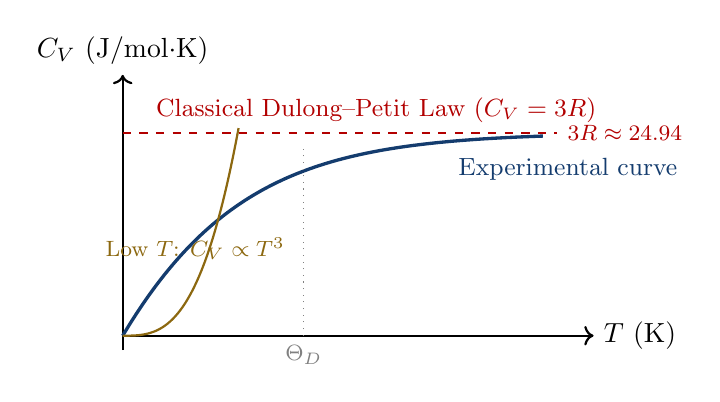
\begin{tikzpicture}[scale=0.92]
  \draw[->,thick] (0,0) -- (6.5,0) node[right] {$T$ (K)};
  \draw[->,thick] (0,-0.2) -- (0,3.6) node[above] {$C_V$ (J/mol$\cdot$K)};

  % Dulong-Petit asymptote
  \draw[dashed,thick,red!70!black] (0,2.8) -- (6.0,2.8) node[right,font=\footnotesize] {$3R \approx 24.94$};

  % Experimental / Real Debye curve
  \draw[ntccblue,very thick,domain=0:5.8,samples=150]
    plot (\x, {2.8*(1 - exp(-0.8*\x) - 0.2*\x*exp(-0.9*\x))});

  % T^3 low-T tangent
  \draw[ntccgold!80!black,thick,domain=0:1.6,samples=60]
    plot (\x, {0.7*\x*\x*\x});
  \node[font=\footnotesize,ntccgold!80!black] at (1.0,1.2) {Low $T$: $C_V \propto T^3$};

  % Annotations
  \node[above,font=\small,red!70!black] at (3.5,2.8) {Classical Dulong--Petit Law ($C_V = 3R$)};
  \node[right,font=\small,ntccblue] at (4.5,2.3) {Experimental curve};
  \draw[dotted,gray] (2.5,0) node[below,font=\footnotesize] {$\Theta_D$} -- (2.5,2.65);
\end{tikzpicture}
\caption{Molar specific heat $C_V(T)$ of a typical non-magnetic dielectric crystal. At high temperatures ($T \gg \Theta_D$), $C_V$ approaches the classical Dulong--Petit limit $3R$. At low temperatures ($T \ll \Theta_D$), quantum freeze-out suppresses $C_V$ with a characteristic $T^3$ power law.}
\label{fig:cv_experimental_vs_classical}
\end{figure}

\subsection{Einstein Model \hfill \small(20 min)}

\textbf{Assumption.} All $3N$ oscillators share the \emph{same} frequency $\omega_E$
(the Einstein frequency).

\textbf{Energy.}
\[
U = 3N\,\frac{\hbar\omega_E}{e^{\hbar\omega_E/k_BT}-1} + \frac{3N\hbar\omega_E}{2}
\quad(\text{zero-point term dropped for } C_V)
\]

\begin{keybox}[Einstein Specific Heat]
\[
C_V = 3Nk_B\left(\frac{\Theta_E}{T}\right)^2\frac{e^{\Theta_E/T}}{\left(e^{\Theta_E/T}-1\right)^2},
\qquad \Theta_E \equiv \frac{\hbar\omega_E}{k_B}
\]
\end{keybox}

\textbf{Limiting behaviour.}
\begin{itemize}
\item High $T$ ($T\gg\Theta_E$): $C_V\to 3Nk_B$ (Dulong--Petit, correct!)
\item Low $T$ ($T\ll\Theta_E$): $C_V\approx 3Nk_B(\Theta_E/T)^2e^{-\Theta_E/T}$ -- exponential decay
\end{itemize}

\textbf{Comparison with experiment.}
\begin{itemize}
\item High $T$: correct.
\item Low $T$: experiment shows $C_V\propto T^3$, but Einstein predicts a faster
(exponential) decay. The discrepancy arises because Einstein ignores the
low-frequency \emph{acoustic} modes.
\end{itemize}

\subsection{Einstein Temperature and Physical Interpretation \hfill \small(10 min)}

\textbf{Typical values.}
\begin{center}
\begin{tabular}{lc}
\toprule
Material & $\Theta_E$ (K)\\
\midrule
Diamond & $\approx 1320$ (very stiff bonds)\\
Copper & $\approx 240$\\
Lead & $\approx 68$ (soft, heavy)\\
\bottomrule
\end{tabular}
\end{center}

\begin{physbox}[Physical meaning]
$\Theta_E$ characterises lattice stiffness: high $\Theta_E$ means stiff bonds,
light atoms, high vibrational frequencies. It is treated as a fitting parameter and
works reasonably well for optical modes, but fails for acoustic modes.
\end{physbox}

\begin{pitbox}[$\Theta_E$ and $\Theta_D$ are not the same number]
For the same material, $\Theta_E$ and $\Theta_D$ are not interchangeable. The
Einstein temperature is set by an optical-mode frequency; the Debye temperature
is a particular average over the acoustic dispersion. Numerically, $\Theta_D$ is
typically 70--80\% of $\Theta_E$ -- a rule of thumb, not an identity.
\end{pitbox}

\subsection{Computational Illustration \hfill \small(10 min)}

\begin{pybox}[Python: Einstein specific heat and the Dulong--Petit limit]
\begin{lstlisting}
import numpy as np
import matplotlib.pyplot as plt
kB = 1.380649e-23
NA = 6.02214076e23
R  = NA*kB

def Cv_Einstein(T, ThetaE):
    x = ThetaE/T
    # numerical guard against T=0
    x = np.where(x > 500, 500, x)
    return 3*R * x**2 * np.exp(x) / (np.exp(x) - 1.0)**2

T = np.linspace(1, 1000, 1000)
for ThetaE in (68, 240, 1320):   # Pb, Cu, diamond
    plt.plot(T, Cv_Einstein(T, ThetaE), label=fr'$\Theta_E={ThetaE}$~K')

plt.axhline(3*R, color='k', ls=':', label='Dulong--Petit 3R')
plt.xscale('log')
plt.xlabel('T (K)'); plt.ylabel(r'$C_V$ (J/mol.K)')
plt.ylim(0, 30); plt.legend()
plt.tight_layout(); plt.show()
\end{lstlisting}
\end{pybox}

\begin{figure}[htbp]
\centering
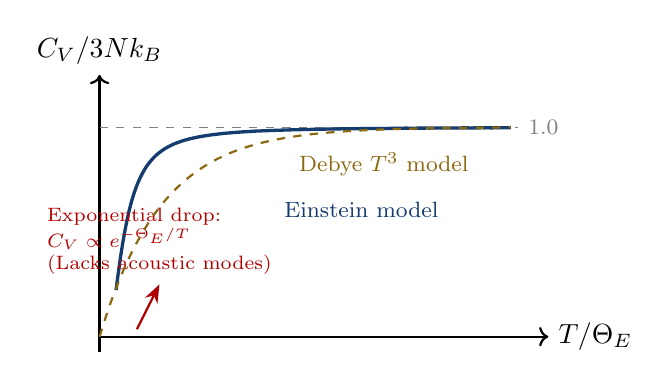
\begin{tikzpicture}[scale=0.95]
  \draw[->,thick] (0,0) -- (6.0,0) node[right] {$T/\Theta_E$};
  \draw[->,thick] (0,-0.2) -- (0,3.5) node[above] {$C_V / 3Nk_B$};

  % Dulong-Petit asymptote
  \draw[dashed,gray] (0,2.8) -- (5.6,2.8) node[right,font=\footnotesize] {$1.0$};

  % Einstein curve: x^2 e^x / (e^x-1)^2 with x = Theta_E/T = 1/t
  \draw[ntccblue,very thick,domain=0.22:5.5,samples=180]
    plot (\x, {2.8 / ( (exp(1.0/\x) - 1.0)*(exp(1.0/\x) - 1.0) ) * (1.0/(\x*\x)) * exp(1.0/\x)});

  % Low-T exponential failure label
  \draw[->,>=Stealth,thick,red!70!black] (0.5,0.1) -- (0.8,0.7)
    node[above,font=\scriptsize,align=left] {Exponential drop:\\$C_V \propto e^{-\Theta_E/T}$\\(Lacks acoustic modes)};

  % Actual T^3 Debye curve comparison (dotted)
  \draw[ntccgold!80!black,thick,dashed,domain=0:5.5,samples=120]
    plot (\x, {2.8*(1 - exp(-1.2*\x))});
  \node[font=\footnotesize,ntccgold!80!black] at (3.8,2.3) {Debye $T^3$ model};
  \node[font=\footnotesize,ntccblue] at (3.5,1.7) {Einstein model};
\end{tikzpicture}
\caption{Dimensionless heat capacity $C_V/3Nk_B$ according to the Einstein model as a function of reduced temperature $T/\Theta_E$. While capturing the high-temperature saturation at $3Nk_B$, it drops off exponentially at low temperatures ($e^{-\Theta_E/T}$), failing to predict the correct experimental $T^3$ acoustic dependence.}
\label{fig:einstein_model_curve}
\end{figure}

\begin{probbox}
\begin{enumerate}
\item Calculate the Einstein temperature for a solid with $\omega_E=10^{13}$~rad/s.
\item Show that the Einstein specific heat approaches $3Nk_B$ at high $T$.
\item At what fraction of $\Theta_E$ does $C_V$ reach 90\% of the Dulong--Petit value?
\end{enumerate}
\end{probbox}

\newpage
% ======================================================================
\lecheader{12}{Debye Model of Specific Heat}{50 minutes}

\begin{keybox}[Learning Objectives]
\begin{itemize}
\item Derive the Debye model using a linear dispersion approximation
\item Understand the Debye temperature and cutoff frequency
\item Reproduce the $T^3$ law at low temperature
\end{itemize}
\end{keybox}

\begin{histbox}[Peter Debye, 1912]
Debye's 1912 paper was a single tidy move: replace the unrealistic single-frequency
assumption with a realistic linear acoustic dispersion $\omega=v_s k$, and let the
cutoff be set by counting modes. The $T^3$ law at low $T$ drops out of the
Debye integral essentially automatically. It is one of the cleanest successes of
early quantum theory.
\end{histbox}

\subsection{Motivation and Assumptions \hfill \small(8 min)}

\textbf{Einstein model failure.} At low $T$, only low-frequency (acoustic) modes are
excited, but the Einstein model treats all modes as high-frequency optical modes.

\textbf{Debye's insight.} At low $T$, only long-wavelength acoustic modes matter, and
these obey a \textbf{linear dispersion}: $\omega=v_sk$.

\textbf{Assumptions.}
\begin{enumerate}
\item Linear dispersion for \emph{all} modes: $\omega=v_sk$.
\item Isotropic solid with an average sound velocity $v_s$.
\item A cutoff frequency $\omega_D$ (Debye frequency) such that the total number of
modes equals $3N$.
\end{enumerate}

\begin{pitbox}[What the Debye model gets wrong]
The Debye model assumes $\omega = v_s k$ up to the cutoff. Real solids have a
\emph{flat} optical-like region near the zone boundary where $v_g$ goes to zero.
This means the true high-$T$ $C_V$ is slightly below $3R$ and the approach to the
limit is not exactly the Dulong--Petit curve. The model is, however, excellent at
low $T$ (where only the linear regime matters) and qualitatively correct at all
temperatures.
\end{pitbox}

\subsection{Density of States in 3D \hfill \small(12 min)}

For a continuous isotropic medium, the number of modes with $|\mathbf k|<k$:
\[
N(k) = \frac{V}{(2\pi)^3}\times\frac{4\pi k^3}{3}\times3 = \frac{Vk^3}{2\pi^2}
\]
(the factor of 3 counts polarisations: 1 longitudinal $+$ 2 transverse).

\textbf{Density of states in $k$-space:}
\[
g(k)\,dk = \frac{Vk^2}{2\pi^2}\,dk
\]
\textbf{Converting to frequency} ($\omega=v_sk$):
\begin{keybox}[3D Debye Density of States]
\[
g(\omega)\,d\omega = \frac{V\omega^2}{2\pi^2v_s^3}\,d\omega
\]
\end{keybox}
With different velocities for longitudinal and transverse modes:
\[
\frac{3}{v_s^3} = \frac{1}{v_l^3}+\frac{2}{v_t^3}
\]

\begin{figure}[htbp]
\centering
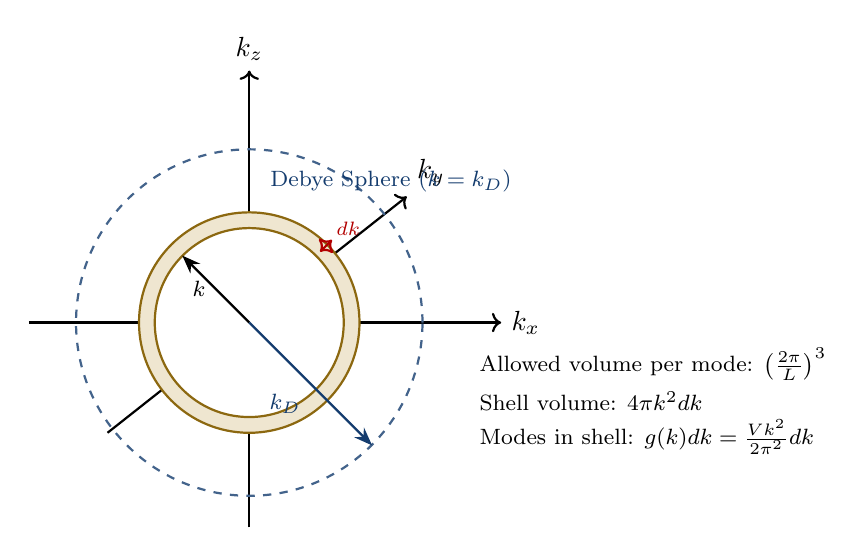
\begin{tikzpicture}[scale=1.0]
  % 3D Axes
  \draw[->,thick] (-2.8,0) -- (3.2,0) node[right] {$k_x$};
  \draw[->,thick] (0,-2.6) -- (0,3.2) node[above] {$k_z$};
  \draw[->,thick] (-1.8,-1.4) -- (2.0,1.6) node[above right] {$k_y$};

  % Debye sphere boundary
  \draw[thick,ntccblue!80,dashed] (0,0) circle (2.2cm);
  \node[ntccblue,font=\footnotesize] at (1.8,1.8) {Debye Sphere ($k = k_D$)};

  % Differential shell
  \draw[fill=ntccgold!20,draw=ntccgold!80!black,thick] (0,0) circle (1.4cm);
  \draw[fill=white,draw=ntccgold!80!black,thick] (0,0) circle (1.2cm);
  \draw[<->,thick,red!70!black] (0.9,0.9) -- (1.05,1.05) node[midway,above right,font=\scriptsize] {$dk$};

  % Radius vector
  \draw[->,>=Stealth,thick,black] (0,0) -- (-0.85,0.85) node[midway,left,font=\footnotesize] {$k$};
  \draw[->,>=Stealth,thick,ntccblue] (0,0) -- (1.56,-1.56) node[midway,below left,font=\footnotesize] {$k_D$};

  % Volume & Mode annotations
  \node[anchor=west,font=\footnotesize,align=left] at (2.8,-1.0) {
    Allowed volume per mode: $\left(\frac{2\pi}{L}\right)^3$\\[3pt]
    Shell volume: $4\pi k^2 dk$\\[3pt]
    Modes in shell: $g(k)dk = \frac{Vk^2}{2\pi^2}dk$
  };
\end{tikzpicture}
\caption{Mode counting in three-dimensional $\mathbf{k}$-space. The differential spherical shell between radius $k$ and $k+dk$ contains $4\pi k^2 dk / (2\pi/L)^3$ spatial modes. The Debye sphere of radius $k_D$ encompasses exactly $3N$ normal vibrational modes.}
\label{fig:kspace_mode_counting}
\end{figure}

\subsection{Debye Cutoff and Specific Heat \hfill \small(15 min)}

\textbf{Debye frequency $\omega_D$}: set the total number of modes equal to $3N$:
\[
\int_0^{\omega_D}g(\omega)\,d\omega = 3N
\ \Longrightarrow\
\frac{V}{2\pi^2v_s^3}\int_0^{\omega_D}\omega^2\,d\omega = 3N
\ \Longrightarrow\
\frac{V\omega_D^3}{6\pi^2v_s^3} = 3N
\]

\textbf{Debye wavevector:}
\[
k_D = \left(\frac{6\pi^2N}{V}\right)^{1/3}
\]
\textbf{Debye temperature:}
\[
\Theta_D = \frac{\hbar\omega_D}{k_B} = \frac{\hbar v_sk_D}{k_B}
\]

\textbf{Specific heat derivation:}
\[
U = \int_0^{\omega_D}\hbar\omega\,\langle n(\omega)\rangle\,g(\omega)\,d\omega
\]
\begin{keybox}[Debye Specific Heat]
\[
C_V = \left(\frac{\partial U}{\partial T}\right)_V
= 9Nk_B\left(\frac{T}{\Theta_D}\right)^3 \int_0^{\Theta_D/T}\frac{x^4e^x}{(e^x-1)^2}\,dx,
\qquad x\equiv\frac{\hbar\omega}{k_BT}
\]
\end{keybox}

\subsection{Limiting Behaviour \hfill \small(10 min)}

\textbf{High $T$ ($T\gg\Theta_D$):} expand $e^x\approx1+x$:
\[
C_V \approx 9Nk_B\left(\frac{T}{\Theta_D}\right)^3\int_0^{\Theta_D/T}x^2\,dx
= 9Nk_B\left(\frac{T}{\Theta_D}\right)^3\cdot\frac13\left(\frac{\Theta_D}{T}\right)^3
= 3Nk_B
\]
$\Rightarrow$ Dulong--Petit law recovered.

\textbf{Low $T$ ($T\ll\Theta_D$):} the upper limit $\Theta_D/T\to\infty$, and
\[
\int_0^\infty \frac{x^4e^x}{(e^x-1)^2}\,dx = \frac{4\pi^4}{15}
\]
\begin{keybox}[Debye $T^3$ Law]
\[
C_V = \frac{12\pi^4}{5}Nk_B\left(\frac{T}{\Theta_D}\right)^3 \ \propto\ T^3
\]
\end{keybox}
This matches experimental data extremely well for non-magnetic insulators.
\textbf{Where the $12\pi^4/5$ comes from:} it is $3 \times 4\pi^4/15$ -- the
factor 3 is the three acoustic polarisations, $4\pi^4/15$ is the standard
Bose--Einstein integral $\int_0^\infty x^4 e^x/(e^x-1)^2\,dx$.

\begin{expbox}[Why low-$T$ $C_V$ is the cleanest test of any phonon model]
The Debye $T^3$ law is so robust that deviations from it are diagnostic. For
example, in glasses the specific heat goes as $C_V \propto T$ (two-level systems)
below ~1~K -- a famous signature of amorphous solids. In ferroelectrics near $T_C$
a ``critical'' contribution appears on top of the Debye $T^3$. Plotting $C_V/T^3$
vs. $T$ is therefore a standard first-look diagnostic in any low-$T$ specific-heat
experiment.
\end{expbox}

\begin{figure}[htbp]
\centering
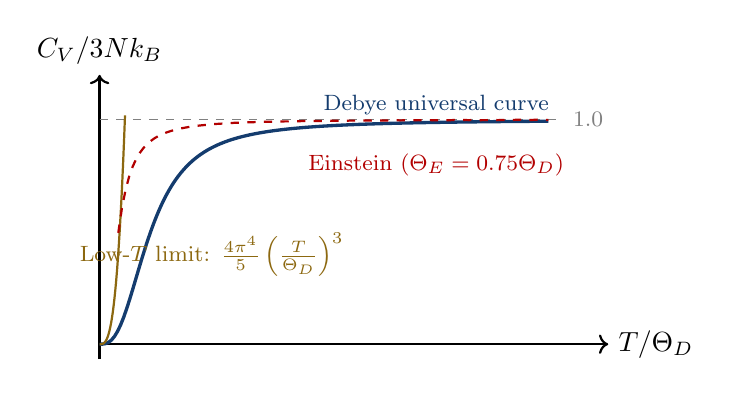
\begin{tikzpicture}[scale=0.95]
  \draw[->,thick] (0,0) -- (6.8,0) node[right] {$T/\Theta_D$};
  \draw[->,thick] (0,-0.2) -- (0,3.6) node[above] {$C_V / 3Nk_B$};

  % Asymptote
  \draw[dashed,gray] (0,3.0) -- (6.2,3.0) node[right,font=\footnotesize] {$1.0$};

  % Debye full curve (numerical approximation)
  \draw[ntccblue,very thick,domain=0:6.0,samples=150]
    plot (\x, {3.0 * (\x*\x*\x) / (\x*\x*\x + 0.18 + 0.2*\x)});

  % Low-T T^3 tangent
  \draw[ntccgold!80!black,thick,domain=0:0.34,samples=30]
    plot (\x, {3.0 * (12.0*3.14159^4/15.0) * (\x^3) / 3.0 });
  \node[font=\footnotesize,ntccgold!80!black] at (1.5,1.2) {Low-$T$ limit: $\frac{4\pi^4}{5}\left(\frac{T}{\Theta_D}\right)^3$};

  % Einstein comparison (dashed red)
  \draw[red!70!black,thick,dashed,domain=0.25:6.0,samples=120]
    plot (\x, {3.0 / ( (exp(0.75/\x) - 1.0)*(exp(0.75/\x) - 1.0) ) * (0.75*0.75/(\x*\x)) * exp(0.75/\x)});
  \node[font=\footnotesize,red!70!black] at (4.5,2.4) {Einstein ($\Theta_E = 0.75\Theta_D$)};
  \node[font=\footnotesize,ntccblue] at (4.5,3.2) {Debye universal curve};
\end{tikzpicture}
\caption{Universal Debye specific heat $C_V / 3Nk_B$ as a function of reduced temperature $T/\Theta_D$. At low temperatures ($T/\Theta_D < 0.1$), the curve follows the exact $T^3$ tangent. The Einstein curve with matched median frequency drops significantly faster at low temperatures.}
\label{fig:debye_universal_specific_heat}
\end{figure}

\begin{keybox}[Summary -- Three Models Compared]
\begin{center}
\renewcommand{\arraystretch}{1.3}
\begin{tabular}{lccc}
\toprule
 & \textbf{Classical} & \textbf{Einstein} & \textbf{Debye}\\
\midrule
Mode frequencies & -- (equipartition) & all $=\omega_E$ & continuum, $\omega=v_sk$, cutoff $\omega_D$\\
High-$T$ limit & $3Nk_B$ & $3Nk_B$ & $3Nk_B$\\
Low-$T$ limit & $3Nk_B$ (wrong) & $\propto e^{-\Theta_E/T}$ & $\propto T^3$ (correct)\\
\bottomrule
\end{tabular}
\end{center}
\end{keybox}

\subsection{Computational Illustration \hfill \small(5 min)}

\begin{pybox}[Python: Debye specific heat, low-$T$ $T^3$, and Einstein overlay]
\begin{lstlisting}
import numpy as np
from scipy.integrate import quad
import matplotlib.pyplot as plt

kB = 1.380649e-23
R  = 8.314462618

def integrand(x):
    return x**4 * np.exp(x) / (np.exp(x) - 1.0)**2

def Cv_Debye(T, ThetaD):
    upper = ThetaD/T if T > 0 else 700
    upper = min(upper, 700)   # numerical cutoff
    val, _ = quad(integrand, 0, upper)
    return 9*R * (T/ThetaD)**3 * val

def Cv_Einstein(T, ThetaE):
    x = ThetaE/T
    return 3*R * x**2 * np.exp(x) / (np.exp(x) - 1.0)**2

T = np.linspace(1, 600, 600)
ThetaD = 320.0  # K
Cv_D = np.array([Cv_Debye(t, ThetaD) for t in T])
Cv_E = Cv_Einstein(T, ThetaD)   # using ThetaD as ThetaE for the overlay

plt.plot(T, Cv_D, label='Debye')
plt.plot(T, Cv_E, '--', label=fr'Einstein, $\Theta_E=\Theta_D$')
plt.axhline(3*R, color='k', ls=':', label='Dulong--Petit')
plt.xlabel('T (K)'); plt.ylabel(r'$C_V$ (J/mol.K)')
plt.legend(); plt.tight_layout(); plt.show()
\end{lstlisting}
\end{pybox}

\begin{probbox}
\begin{enumerate}
\item Calculate the Debye temperature for copper given $v_l=4760$~m/s,
$v_t=2325$~m/s, and atomic density $n=8.5\times10^{28}$~m$^{-3}$.
\item Show that the Debye model reduces to Dulong--Petit at high $T$.
\item At $T=10$~K, calculate the specific heat of Al ($\Theta_D=394$~K) using the
Debye model.
\end{enumerate}
\end{probbox}

\newpage
% ======================================================================
\lecheader{13}{Thermal Conductivity of Insulators}{50 minutes}

\begin{keybox}[Learning Objectives]
\begin{itemize}
\item Understand the kinetic theory of thermal conductivity
\item Derive the phonon thermal conductivity formula
\item Explain the role of phonon scattering mechanisms
\end{itemize}
\end{keybox}

\begin{expbox}[What $\kappa(T)$ actually looks like]
The thermal conductivity of pure dielectric crystals (e.g.\ NaF, sapphire, diamond)
is one of the most striking non-monotonic curves in solid-state physics. At the
lowest $T$, $\kappa\propto T^3$ (specific heat rising, mean free path set by the
sample size -- Casimir regime). It peaks at a few percent of $\Theta_D$, then
falls as $1/T$ at high $T$ (Umklapp-dominated). The peak value can exceed
$10^4$~W/m$\cdot$K in isotopically pure diamond at low $T$ -- the highest thermal
conductivity of any known solid.
\end{expbox}

\subsection{Kinetic Theory Approach \hfill \small(12 min)}

\textbf{Thermal conductivity from kinetic theory:}
\[
\kappa = \frac13C_Vv\ell
\]
where $C_V$ is the specific heat per unit volume, $v$ the particle velocity, and
$\ell$ the mean free path.

\textbf{For phonons:}
\begin{keybox}[Phonon Thermal Conductivity]
\[
\kappa = \frac13C_Vv_s\ell
\]
\end{keybox}

\begin{physbox}
Heat flows because phonons with higher energy (from the hot side) diffuse toward the
cold side. The mean free path $\ell$ is limited by scattering processes.
\end{physbox}

\subsection{Phonon Scattering Mechanisms \hfill \small(18 min)}

\textbf{1. Phonon--phonon scattering (Umklapp processes).}
At high $T$, phonon density is high $\Rightarrow$ frequent collisions. Only Umklapp
processes (which change total crystal momentum) contribute to thermal resistance.

Temperature dependence:
\begin{itemize}
\item High $T$: $\ell\propto1/T$ (phonon density $\propto T$) $\Rightarrow \kappa\propto1/T$ (since $C_V$ is constant at high $T$).
\end{itemize}

\textbf{2. Boundary scattering.} At low $T$, the phonon mean free path is limited by
sample dimensions:
\[
\ell \approx L\ (\text{sample size}), \qquad \kappa = \frac13C_Vv_sL \propto T^3
\]

\textbf{3. Impurity/defect scattering.} Point defects, isotopes and dislocations
scatter phonons. At low $T$:
\[
\ell \propto 1/\omega^4 \propto 1/T^4 \qquad (\text{Rayleigh scattering, } \sigma\propto\omega^4)
\]

\textbf{4. Electron--phonon scattering.} In metals, electrons also scatter and are
scattered by phonons.

\begin{figure}[h]
\centering
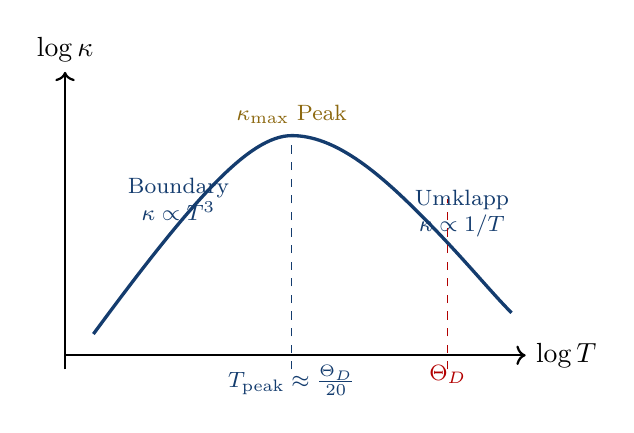
\begin{tikzpicture}[scale=0.9]
  % log-log axes
  \draw[->,thick] (0,0) -- (6.5,0) node[right] {$\log T$};
  \draw[->,thick] (0,-0.2) -- (0,4.0) node[above] {$\log \kappa$};
  % the schematic curve: T^3 up (boundary), peak at T ~ Theta_D/20, Umklapp 1/T falloff
  \draw[ntccblue,very thick]
    (0.4,0.3) .. controls (1.8,2.2) and (2.6,3.1) .. (3.2,3.1)
              .. controls (3.8,3.1) and (4.4,2.6) .. (5.0,2.0)
              .. controls (5.6,1.4) and (6.0,0.9) .. (6.3,0.6);
  % region labels
  \node[font=\footnotesize,ntccblue,align=center] at (1.6,2.2) {Boundary\\$\kappa \propto T^3$};
  \node[font=\footnotesize,ntccblue,align=center] at (5.6,2.0) {Umklapp\\$\kappa \propto 1/T$};
  \node[font=\footnotesize,ntccgold!80!black,align=center] at (3.2,3.4) {$\kappa_{\max}$ Peak};
  % Peak marker and Theta_D marker
  \draw[ntccblue,dashed] (3.2,-0.2) -- (3.2,3.1);
  \node[font=\footnotesize,ntccblue,below] at (3.2,0) {$T_{\text{peak}} \approx \frac{\Theta_D}{20}$};
  \draw[red!70!black,dashed] (5.4,-0.2) -- (5.4,2.2);
  \node[font=\footnotesize,red!70!black,below] at (5.4,0) {$\Theta_D$};
\end{tikzpicture}
\caption{Schematic $\kappa(T)$ for a pure dielectric crystal on log--log axes.
Three regimes: $T^3$ (boundary-limited), peak near $T\approx\Theta_D/20$, then
$1/T$ (Umklapp-limited).}
\end{figure}

\subsection{Debye--Peierls Theory \hfill \small(12 min)}

\textbf{Peierls' contribution.} Normal phonon processes ($\mathbf G=0$) do not
contribute to thermal resistance because total crystal momentum is conserved. Only
Umklapp processes create resistance.

\textbf{Umklapp condition.} At least one phonon must have $k>\pi/2a$ (half the zone
boundary). The probability of such high-$k$ phonons:
\[
P \propto e^{-\Theta_D/2T}
\]

\begin{keybox}[Resulting Thermal Conductivity]
\[
\kappa \propto e^{\Theta_D/2T} \ \ (\text{intermediate } T); \qquad
\kappa\propto1/T \ (\text{high } T); \qquad
\kappa\propto T^3 \ (\text{low } T,\text{ boundary limited})
\]
\end{keybox}

\subsection{Computational Illustration \hfill \small(5 min)}

\begin{pybox}[Python: Matthiessen's-rule model of $\kappa(T)$]
\begin{lstlisting}
import numpy as np
import matplotlib.pyplot as plt

# Simple model: combine boundary (Casimir) and Umklapp
# kappa(T) = (1/3) * Cv(T) * v_s * l_eff,  l_eff^-1 = l_b^-1 + l_U^-1

def Cv_Debye_per_vol(T, ThetaD, rho):
    # approximate low-T Cv ~ (12 pi^4 / 5) * (N/V) * kB * (T/ThetaD)^3
    n = rho / (40*1.66e-27)   # for 40 amu, e.g. Ca-like
    a = 12*np.pi**4/5 * n * 1.38e-23 * (T/ThetaD)**3
    return np.where(T < ThetaD/2, a, 3*n*1.38e-23)   # plateau at Dulong-Petit

v_s   = 4000.0
rho   = 3000.0
ThetaD= 300.0
L     = 1e-3   # 1 mm sample

T = np.linspace(1, 500, 500)
Cv  = Cv_Debye_per_vol(T, ThetaD, rho)
l_b = L*np.ones_like(T)
l_U = (1e-2) * (ThetaD/T)        # crude Umklapp MFP, ~ 10 microns at T=ThetaD
l_eff = 1.0/(1.0/l_b + 1.0/l_U)
kappa = (1.0/3.0) * Cv * v_s * l_eff

plt.loglog(T, kappa)
plt.xlabel('T (K)'); plt.ylabel(r'$\kappa$ (W/m.K)')
plt.title('Matthiessen model: boundary + Umklapp')
plt.tight_layout(); plt.show()
\end{lstlisting}
\end{pybox}

\begin{probbox}
\begin{enumerate}
\item Estimate the phonon mean free path in diamond at room temperature given
$\kappa=2000$~W/m$\cdot$K, $v_s=12000$~m/s, and $C_V=1.8\times10^6$~J/m$^3\cdot$K.
\item Why does the thermal conductivity of amorphous solids not show $T^3$ behaviour
at low $T$?
\item Explain the role of isotope scattering in reducing thermal conductivity.
\end{enumerate}
\end{probbox}

\newpage
% ======================================================================
\lecheader{14}{Lattice Vibrations in 2D and 3D}{50 minutes}

\begin{keybox}[Learning Objectives]
\begin{itemize}
\item Extend lattice dynamics to higher dimensions
\item Understand polarisation and the number of branches
\item Calculate the density of states in 2D and 3D
\end{itemize}
\end{keybox}

\subsection{3D Monoatomic Lattice \hfill \small(15 min)}

\textbf{Setup.} $N$ atoms in a 3D Bravais lattice, each with 3 degrees of freedom
$\Rightarrow 3N$ normal modes.

\textbf{Dispersion relation.} For each $\mathbf k$ in the first Brillouin zone there
are \textbf{3 branches}:
\begin{itemize}
\item 1 longitudinal acoustic (LA) branch
\item 2 transverse acoustic (TA) branches
\end{itemize}

\textbf{Equations of motion:}
\[
M\frac{d^2u_\alpha(\mathbf R)}{dt^2} = -\sum_{\mathbf R'}\sum_\beta\Phi_{\alpha\beta}(\mathbf R-\mathbf R')\,u_\beta(\mathbf R')
\]
where $\Phi_{\alpha\beta}$ is the force-constant matrix.

\textbf{Dynamical matrix:}
\[
D_{\alpha\beta}(\mathbf k) = \frac1M\sum_{\mathbf R}\Phi_{\alpha\beta}(\mathbf R)\,e^{-i\mathbf k\cdot\mathbf R}
\]
The eigenvalues of $D_{\alpha\beta}(\mathbf k)$ give $\omega^2(\mathbf k)$ for the
three branches.

\begin{figure}[htbp]
\centering
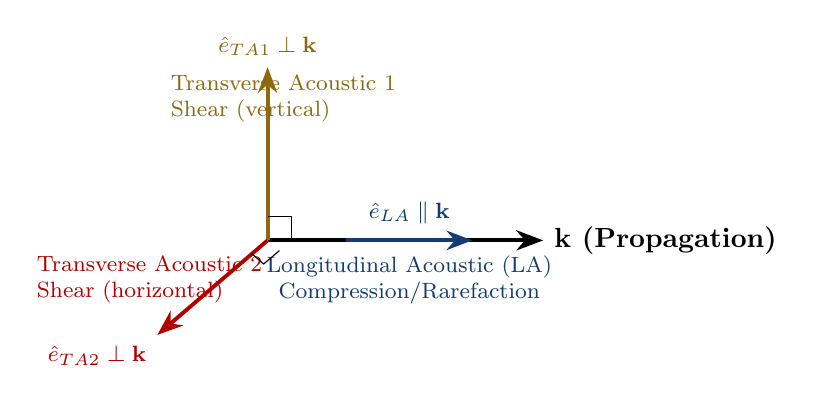
\begin{tikzpicture}[scale=1.0]
  % Wavevector k
  \draw[->,>=Stealth,line width=1.5pt,black] (0,0) -- (3.5,0) node[right,font=\bfseries] {$\mathbf{k}$ (Propagation)};

  % Longitudinal polarization vector
  \draw[->,>=Stealth,line width=1.4pt,ntccblue] (1.0,0) -- (2.6,0) node[midway,above=2pt,font=\footnotesize] {$\hat{e}_{LA} \parallel \mathbf{k}$};
  \node[font=\footnotesize,ntccblue,align=center] at (1.8,-0.5) {Longitudinal Acoustic (LA)\\Compression/Rarefaction};

  % Transverse polarization 1 (in-plane y)
  \draw[->,>=Stealth,line width=1.4pt,ntccgold!80!black] (0,0) -- (0,2.2) node[above,font=\footnotesize] {$\hat{e}_{TA1} \perp \mathbf{k}$};
  \node[font=\footnotesize,ntccgold!80!black,align=left] at (0.2,1.8) {Transverse Acoustic 1\\Shear (vertical)};

  % Transverse polarization 2 (out-of-plane z)
  \draw[->,>=Stealth,line width=1.4pt,red!70!black] (0,0) -- (-1.4,-1.2) node[below left,font=\footnotesize] {$\hat{e}_{TA2} \perp \mathbf{k}$};
  \node[font=\footnotesize,red!70!black,align=left] at (-1.5,-0.5) {Transverse Acoustic 2\\Shear (horizontal)};

  % Orthogonality markers
  \draw (0.3,0) -- (0.3,0.3) -- (0,0.3);
  \draw (-0.2,-0.17) -- (-0.05,-0.3) -- (0.15,-0.13);
\end{tikzpicture}
\caption{Polarization eigenvectors for acoustic vibrational waves in a three-dimensional continuum. For each wavevector $\mathbf{k}$, there are three mutually orthogonal acoustic modes: one longitudinal wave ($\hat{e}_{LA} \parallel \mathbf{k}$) and two transverse waves ($\hat{e}_{TA1}, \hat{e}_{TA2} \perp \mathbf{k}$).}
\label{fig:phonon_polarization_vectors}
\end{figure}

\subsection{3D Diatomic Lattice \hfill \small(12 min)}

\textbf{Setup.} Basis of 2 atoms per primitive cell $\Rightarrow 6N$ normal modes
($3\times2N$ atoms).

\textbf{Branches.}
\begin{itemize}
\item 3 acoustic branches (1 LA $+$ 2 TA)
\item 3 optical branches (1 LO $+$ 2 TO)
\end{itemize}

\textbf{LO--TO splitting.} In polar crystals (ionic bonds), the longitudinal optical
(LO) and transverse optical (TO) modes differ in frequency at $\mathbf k=0$ due to
long-range electrostatic forces:
\begin{keybox}[Lyddane--Sachs--Teller Relation]
\[
\omega_{LO}^2-\omega_{TO}^2 = \frac{ne^2}{\mu\epsilon_0\epsilon_\infty}
\]
where $\mu$ is the reduced mass and $\epsilon_\infty$ the high-frequency dielectric
constant.
\end{keybox}

\begin{pitbox}[Lyddane--Sachs--Teller is only at $\mathbf k=0$ and only for polar crystals]
The LST relation $\omega_{LO}^2/\omega_{TO}^2 = \epsilon_0/\epsilon_\infty$ (in the
simpler form) holds \emph{only} at $\mathbf k=0$ and \emph{only} when the
long-range Coulomb interaction between ions lifts the LO--TO degeneracy. It does
\emph{not} apply in non-polar crystals (Si, Ge, diamond) where LO and TO are
degenerate at $\mathbf k=0$.
\end{pitbox}

\subsection{Density of States in 2D and 3D \hfill \small(13 min)}

\textbf{General formula:}
\[
g(\omega) = \sum_s\int_{BZ}\frac{d^dk}{(2\pi)^d}\,\delta\!\left(\omega-\omega_s(\mathbf k)\right)
\]

\textbf{3D:}
\[
g(\omega) = \frac{V}{2\pi^2}\sum_s\frac{k^2}{|v_{gs}|}, \qquad
g(\omega)\propto\omega^2 \ \ \text{(isotropic linear dispersion)}
\]
\textbf{2D:}
\[
g(\omega) = \frac{A}{2\pi}\sum_s\frac{k}{|v_{gs}|}, \qquad
g(\omega)\propto\omega \ \ \text{(isotropic linear dispersion)}
\]
\textbf{1D (recap):}
\[
g(\omega) = \frac{L}{\pi}\sum_s\frac{1}{|v_{gs}|}
\]

\begin{keybox}[Dimensional pattern]
$g(\omega)\propto\omega^{d-1}$ for a linear, isotropic dispersion in $d$ dimensions
-- a useful mnemonic linking the 1D, 2D and 3D results above.
\end{keybox}

\textbf{Van Hove singularities.} These occur at critical points where
$v_g=d\omega/dk=0$ (stationary points of the dispersion). $g(\omega)$ diverges or has
discontinuous derivatives there.

\begin{figure}[htbp]
\centering
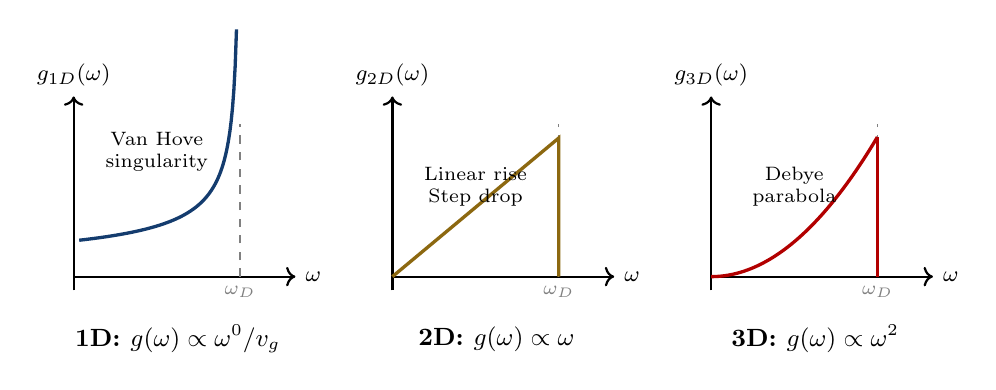
\begin{tikzpicture}[scale=0.88]
  % 1D DOS
  \begin{scope}[xshift=0cm]
    \draw[->,thick] (0,0) -- (3.2,0) node[right,font=\footnotesize] {$\omega$};
    \draw[->,thick] (0,-0.2) -- (0,2.6) node[above,font=\footnotesize] {$g_{1D}(\omega)$};
    \draw[dashed,gray] (2.4,0) node[below,font=\scriptsize] {$\omega_D$} -- (2.4,2.2);
    \draw[ntccblue,very thick,domain=0.08:2.35,samples=120]
      plot (\x, {0.8/sqrt(2.4 - \x)});
    \node[font=\bfseries\small] at (1.5,-0.9) {1D: $g(\omega) \propto \omega^0 / v_g$};
    \node[font=\scriptsize,align=center] at (1.2,1.8) {Van Hove\\singularity};
  \end{scope}

  % 2D DOS
  \begin{scope}[xshift=4.6cm]
    \draw[->,thick] (0,0) -- (3.2,0) node[right,font=\footnotesize] {$\omega$};
    \draw[->,thick] (0,-0.2) -- (0,2.6) node[above,font=\footnotesize] {$g_{2D}(\omega)$};
    \draw[dashed,gray] (2.4,0) node[below,font=\scriptsize] {$\omega_D$} -- (2.4,2.2);
    \draw[ntccgold!80!black,very thick] (0,0) -- (2.4,2.0) -- (2.4,0);
    \node[font=\bfseries\small] at (1.5,-0.9) {2D: $g(\omega) \propto \omega$};
    \node[font=\scriptsize,align=center] at (1.2,1.3) {Linear rise\\Step drop};
  \end{scope}

  % 3D DOS
  \begin{scope}[xshift=9.2cm]
    \draw[->,thick] (0,0) -- (3.2,0) node[right,font=\footnotesize] {$\omega$};
    \draw[->,thick] (0,-0.2) -- (0,2.6) node[above,font=\footnotesize] {$g_{3D}(\omega)$};
    \draw[dashed,gray] (2.4,0) node[below,font=\scriptsize] {$\omega_D$} -- (2.4,2.2);
    \draw[red!70!black,very thick,domain=0:2.4,samples=80]
      plot (\x, {0.35*\x*\x});
    \draw[red!70!black,very thick] (2.4,2.016) -- (2.4,0);
    \node[font=\bfseries\small] at (1.5,-0.9) {3D: $g(\omega) \propto \omega^2$};
    \node[font=\scriptsize,align=center] at (1.2,1.3) {Debye\\parabola};
  \end{scope}
\end{tikzpicture}
\caption{Comparison of phonon density of states $g(\omega) \propto \omega^{d-1}$ for isotropic linear dispersion in $d = 1, 2, 3$ dimensions. (Left) 1D chain exhibiting inverse square-root Van Hove singularity. (Center) 2D membrane exhibiting linear frequency dependence and discontinuous step at cutoff. (Right) 3D Debye continuum exhibiting parabolic $\omega^2$ dependence.}
\label{fig:phonon_dos_dimensionality}
\end{figure}

\subsection{Computational Illustration \hfill \small(10 min)}

For a 2D square lattice with nearest-neighbour springs, the (simplified isotropic)
dispersion is
\[
\omega(\mathbf k) = \sqrt{\tfrac{2C}{M}\left(2-\cos k_xa-\cos k_ya\right)}.
\]
Plotting $\omega$ along the high-symmetry path $\Gamma\to X\to M\to\Gamma$ produces a
standard ``phonon band structure'' plot; plotting the full 3D surface
$\omega(k_x,k_y)$ over the square Brillouin zone shows the saddle point at $X$ that
produces a Van Hove singularity in $g(\omega)$.

\begin{pybox}[Python: 2D square-lattice dispersion along $\Gamma$--X--M--$\Gamma$]
\begin{lstlisting}
import numpy as np
import matplotlib.pyplot as plt

# 2D square lattice dispersion (C = M = a = 1, arbitrary units)
def omega2D(kx, ky):
    return 2.0*(2.0 - np.cos(kx) - np.cos(ky))

# high-symmetry path:  G(0,0) -> X(pi,0) -> M(pi,pi) -> G(0,0)
def kpath(t):
    # t in [0,1]; 0..0.25 -> G->X, 0.25..0.5 -> X->M, 0.5..1 -> M->G
    if t < 0.25:
        s = t/0.25
        return np.array([np.pi*s, 0.0])
    elif t < 0.5:
        s = (t-0.25)/0.25
        return np.array([np.pi, np.pi*s])
    else:
        s = (t-0.5)/0.5
        return np.array([np.pi*(1-s), np.pi*(1-s)])

t = np.linspace(0, 1, 400)
ks = np.array([kpath(ti) for ti in t])
om = np.sqrt(omega2D(ks[:,0], ks[:,1]))

plt.plot(t, om)
xticks = [0, 0.25, 0.5, 1.0]
xlabels = [r'$\Gamma$', 'X', 'M', r'$\Gamma$']
plt.xticks(xticks, xlabels)
plt.ylabel(r'$\omega(\mathbf k)$')
plt.title('2D square-lattice phonon dispersion')
plt.tight_layout(); plt.show()
\end{lstlisting}
\end{pybox}

\begin{figure}[htbp]
\centering
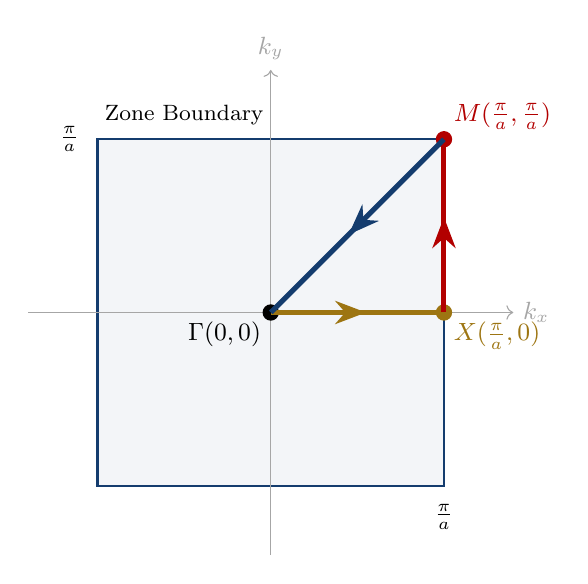
\begin{tikzpicture}[scale=1.1]
  % First Brillouin Zone Square
  \draw[fill=ntccblue!5,draw=ntccblue,thick] (-2,-2) rectangle (2,2);
  \draw[->,gray!70] (-2.8,0) -- (2.8,0) node[right,font=\small] {$k_x$};
  \draw[->,gray!70] (0,-2.8) -- (0,2.8) node[above,font=\small] {$k_y$};

  % High symmetry points
  \filldraw[black] (0,0) circle (2.5pt) node[below left,font=\bfseries\small] {$\Gamma (0,0)$};
  \filldraw[ntccgold!90!black] (2,0) circle (2.5pt) node[below right,font=\bfseries\small] {$X (\frac{\pi}{a},0)$};
  \filldraw[red!70!black] (2,2) circle (2.5pt) node[above right,font=\bfseries\small] {$M (\frac{\pi}{a},\frac{\pi}{a})$};

  % Directed path
  \draw[->,>=Stealth,line width=1.8pt,ntccgold!90!black] (0,0) -- (1.1,0);
  \draw[line width=1.8pt,ntccgold!90!black] (1.0,0) -- (2,0);

  \draw[->,>=Stealth,line width=1.8pt,red!70!black] (2,0) -- (2,1.1);
  \draw[line width=1.8pt,red!70!black] (2,1.0) -- (2,2);

  \draw[->,>=Stealth,line width=1.8pt,ntccblue] (2,2) -- (0.9,0.9);
  \draw[line width=1.8pt,ntccblue] (1.0,1.0) -- (0,0);

  % BZ Boundary labels
  \node[below,font=\footnotesize] at (2,-2.1) {$\frac{\pi}{a}$};
  \node[left,font=\footnotesize] at (-2.1,2) {$\frac{\pi}{a}$};
  \node[above,font=\footnotesize] at (-1.0,2.05) {Zone Boundary};
\end{tikzpicture}
\caption{The first Brillouin zone of a 2D square lattice with lattice constant $a$. The irreducible high-symmetry path $\Gamma(0,0) \to X(\frac{\pi}{a},0) \to M(\frac{\pi}{a},\frac{\pi}{a}) \to \Gamma(0,0)$ spans all independent vibrational wavevectors.}
\label{fig:square_bz_high_symmetry_path}
\end{figure}

\begin{probbox}
\begin{enumerate}
\item How many acoustic and optical branches does a 3D crystal with 4 atoms per
primitive cell have?
\item Derive the DOS for a 2D Debye model and show $C_V\propto T^2$ at low $T$.
\item Explain why graphene has a linear dispersion near the $K$ points (Dirac cones).
\end{enumerate}
\end{probbox}

\newpage
% ======================================================================
\lecheader{15}{Anharmonic Effects and Thermal Expansion}{50 minutes}

\begin{keybox}[Learning Objectives]
\begin{itemize}
\item Understand the origin of thermal expansion
\item Derive the Gr\"uneisen parameter
\item Connect anharmonicity to thermal conductivity
\end{itemize}
\end{keybox}

\begin{histbox}[Eigenvalue Gr\"uneisen, 1926]
Eduard Gr\"uneisen introduced the dimensionless parameter $\gamma$ in 1926 to
relate thermal expansion to specific heat. The relation $\beta = \gamma C_V/(3B)$
is so robust that $\gamma$ is tabulated for essentially every solid. Negative
thermal expansion (Lec 15 problem) was conclusively observed in ZrW$_2$O$_8$ by
Mary et al.\ in 1996 -- a 70-year-old prediction.
\end{histbox}

\subsection{Beyond the Harmonic Approximation \hfill \small(10 min)}

\textbf{Harmonic approximation limitation.} In the harmonic model, phonons do not
interact. This predicts (all wrongly):
\begin{itemize}
\item Infinite thermal conductivity (no phonon--phonon scattering)
\item No thermal expansion (symmetric potential)
\item Elastic constants independent of temperature
\end{itemize}
All three are violated in reality due to \textbf{anharmonicity} (higher-order terms
in the potential).

\textbf{Anharmonic potential:}
\[
U = U_0 + \frac12C_2x^2 + \frac{1}{3!}C_3x^3 + \frac{1}{4!}C_4x^4 + \cdots
\]
The cubic term $C_3x^3$ is the leading anharmonic correction.

\begin{figure}[h]
\centering
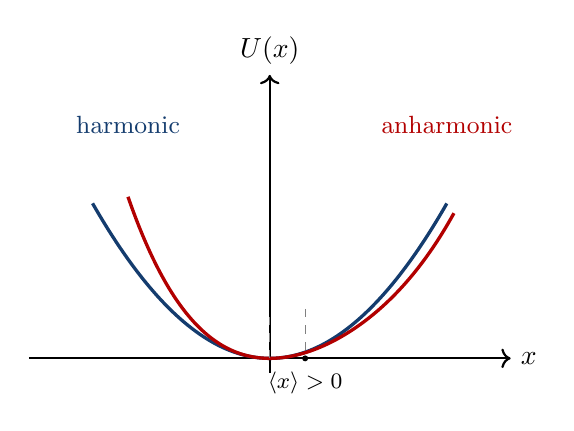
\begin{tikzpicture}[scale=0.9]
  % axes
  \draw[->,thick] (-3.4,0) -- (3.4,0) node[right] {$x$};
  \draw[->,thick] (0,-0.2) -- (0,4.0) node[above] {$U(x)$};
  % harmonic (symmetric)
  \draw[ntccblue,very thick,domain=-2.5:2.5,samples=120] plot (\x, {0.5*0.7*\x*\x});
  \node[ntccblue,font=\small] at (-2.0,3.3) {harmonic};
  % anharmonic (asymmetric)
  \draw[red!70!black,very thick,domain=-2.0:2.6,samples=120]
    plot (\x, {0.5*0.7*\x*\x - 0.07*\x*\x*\x + 0.02*\x*\x*\x*\x});
  \node[red!70!black,font=\small] at (2.5,3.3) {anharmonic};
  % equilibrium mark
  \draw[gray,dashed] (0,0) -- (0,0.7);
  \draw[gray,dashed] (0.5,0.7) -- (0.5,0);
  \fill (0.5,0) circle (1.2pt);
  \node[font=\footnotesize,below] at (0.5,-0.05) {$\langle x\rangle>0$};
\end{tikzpicture}
\caption{Harmonic (symmetric) vs.\ anharmonic (asymmetric) potential. The
anharmonic potential well has a flatter right wall ($x > 0$) due to the negative
cubic term ($-c x^3$) and a steeper left wall ($x < 0$), causing the thermal equilibrium
displacement to expand toward positive separations ($\langle x\rangle > 0$).}
\end{figure}

\subsection{Thermal Expansion \hfill \small(15 min)}

\begin{physbox}[Physical origin]
In a symmetric (harmonic) potential the average position of an oscillator sits at
the minimum regardless of its energy. In an asymmetric (anharmonic) potential,
higher-energy states have their average position shifted to larger separations.
\end{physbox}

\textbf{Gr\"uneisen model.} The Gr\"uneisen parameter $\gamma$ relates thermal
expansion to phonon frequencies:
\begin{keybox}[Gr\"uneisen Parameter]
\[
\gamma = -\frac{d\ln\omega}{d\ln V}
\]
\end{keybox}
For a mode with frequency $\omega$:
\[
\omega = \omega_0 - \gamma\omega_0\frac{\Delta V}{V}
\]

\textbf{Thermal expansion coefficient:}
\[
\beta = \frac1V\left(\frac{\partial V}{\partial T}\right)_P = \frac{\gamma C_V}{3B}
\]
where $B$ is the bulk modulus.

\textbf{Key results.}
\begin{itemize}
\item Low $T$: $\beta\propto T^3$ (since $C_V\propto T^3$).
\item High $T$: $\beta\approx$ constant (since $C_V\approx3Nk_B$).
\end{itemize}

\subsection{Phonon--Phonon Interactions \hfill \small(15 min)}

\textbf{Three-phonon processes.} The cubic anharmonic term allows three-phonon
interactions,
\[
\omega_1+\omega_2=\omega_3
\]
with momentum conservation (normal or Umklapp).

\textbf{Normal processes} ($\mathbf k_1+\mathbf k_2=\mathbf k_3$):
\begin{itemize}
\item Do not contribute to thermal resistance.
\item Redistribute energy among modes but conserve total crystal momentum.
\end{itemize}

\textbf{Umklapp processes} ($\mathbf k_1+\mathbf k_2=\mathbf k_3+\mathbf G$):
\begin{itemize}
\item Change total crystal momentum.
\item Dominant source of thermal resistance at high $T$.
\item Require high-energy phonons ($k>\pi/2a$).
\item Freeze out exponentially at low $T$: $\tau_U^{-1}\propto Te^{-\Theta_D/3T}$.
\end{itemize}

\begin{figure}[htbp]
\centering
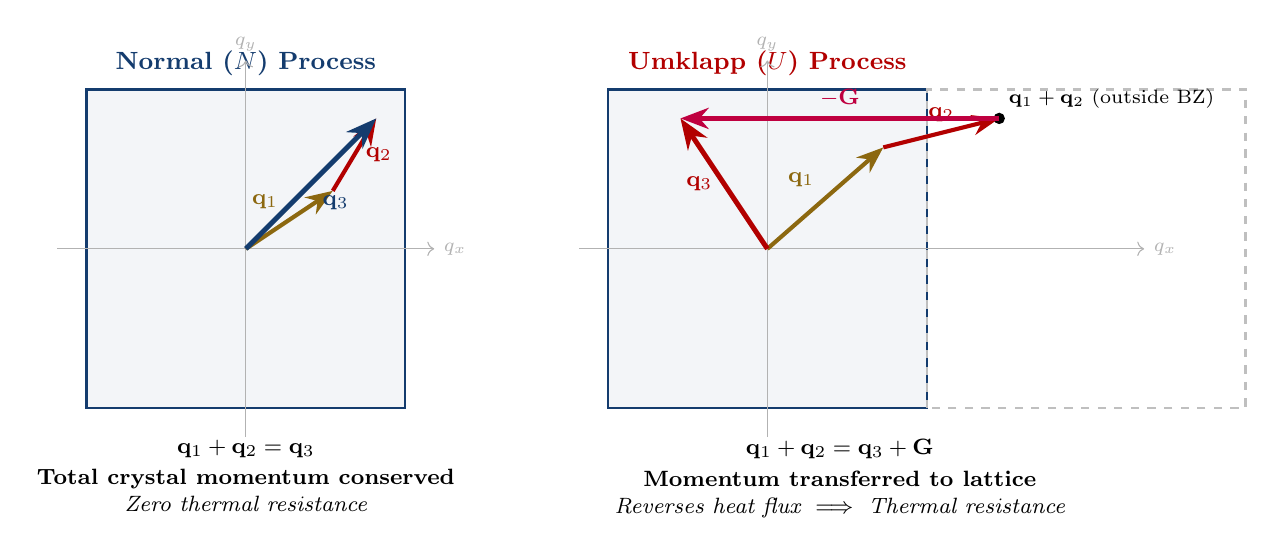
\begin{tikzpicture}[scale=0.92]
  % (a) Normal Process
  \begin{scope}[xshift=0cm]
    \draw[thick,ntccblue,fill=ntccblue!5] (-2.2,-2.2) rectangle (2.2,2.2);
    \node[above,font=\bfseries\small,ntccblue] at (0,2.25) {Normal ($N$) Process};
    \draw[->,gray!60] (-2.6,0) -- (2.6,0) node[right,font=\scriptsize] {$q_x$};
    \draw[->,gray!60] (0,-2.6) -- (0,2.6) node[above,font=\scriptsize] {$q_y$};

    \draw[->,>=Stealth,line width=1.5pt,ntccgold!80!black] (0,0) -- (1.2,0.8) node[midway,above left,font=\footnotesize] {$\mathbf{q}_1$};
    \draw[->,>=Stealth,line width=1.5pt,red!70!black] (1.2,0.8) -- (1.8,1.8) node[midway,right,font=\footnotesize] {$\mathbf{q}_2$};
    \draw[->,>=Stealth,line width=1.8pt,ntccblue] (0,0) -- (1.8,1.8) node[midway,below right,font=\footnotesize] {$\mathbf{q}_3$};

    \node[below,font=\footnotesize,align=center] at (0,-2.5) {$\mathbf{q}_1 + \mathbf{q}_2 = \mathbf{q}_3$\\[2pt]\textbf{Total crystal momentum conserved}\\\itshape Zero thermal resistance};
  \end{scope}

  % (b) Umklapp Process
  \begin{scope}[xshift=7.2cm]
    % Central and adjacent BZ
    \draw[thick,ntccblue,fill=ntccblue!5] (-2.2,-2.2) rectangle (2.2,2.2);
    \draw[thick,gray!50,dashed] (2.2,-2.2) rectangle (6.6,2.2);
    \node[above,font=\bfseries\small,red!70!black] at (0,2.25) {Umklapp ($U$) Process};
    \draw[->,gray!60] (-2.6,0) -- (5.2,0) node[right,font=\scriptsize] {$q_x$};
    \draw[->,gray!60] (0,-2.6) -- (0,2.6) node[above,font=\scriptsize] {$q_y$};

    \draw[->,>=Stealth,line width=1.5pt,ntccgold!80!black] (0,0) -- (1.6,1.4) node[midway,above left,font=\footnotesize] {$\mathbf{q}_1$};
    \draw[->,>=Stealth,line width=1.5pt,red!70!black] (1.6,1.4) -- (3.2,1.8) node[midway,above,font=\footnotesize] {$\mathbf{q}_2$};

    % Sum lands outside
    \filldraw[black] (3.2,1.8) circle (2pt) node[above right,font=\scriptsize] {$\mathbf{q}_1+\mathbf{q}_2$ (outside BZ)};
    % Reciprocal lattice vector G
    \draw[->,>=Stealth,line width=1.6pt,purple] (3.2,1.8) -- (-1.2,1.8) node[midway,above,font=\footnotesize] {$-\mathbf{G}$};
    \draw[->,>=Stealth,line width=1.8pt,red!70!black] (0,0) -- (-1.2,1.8) node[midway,left,font=\footnotesize] {$\mathbf{q}_3$};

    \node[below,font=\footnotesize,align=center] at (1.0,-2.5) {$\mathbf{q}_1 + \mathbf{q}_2 = \mathbf{q}_3 + \mathbf{G}$\\[2pt]\textbf{Momentum transferred to lattice}\\\itshape Reverses heat flux $\implies$ Thermal resistance};
  \end{scope}
\end{tikzpicture}
\caption{Comparison of three-phonon scattering geometries in reciprocal space. (Left) Normal ($N$) process: sum vector $\mathbf{q}_3$ remains inside the first Brillouin zone; total phonon momentum is conserved and heat continues forward unimpeded. (Right) Umklapp ($U$) process: the sum lands outside the first Brillouin zone and is folded back by reciprocal lattice vector $\mathbf{G}$, flipping the net phonon group velocity and creating finite thermal resistance.}
\label{fig:normal_vs_umklapp_scattering}
\end{figure}

\subsection{Gr\"uneisen Parameter and Equation of State \hfill \small(7 min)}

\textbf{Mode Gr\"uneisen parameter:}
\[
\gamma_{\mathbf ks} = -\frac{V}{\omega_{\mathbf ks}}\frac{\partial\omega_{\mathbf ks}}{\partial V}
\]
\textbf{Average Gr\"uneisen parameter:}
\[
\gamma = \frac{\sum_{\mathbf ks}\gamma_{\mathbf ks}C_{\mathbf ks}}{\sum_{\mathbf ks}C_{\mathbf ks}}
\]
\begin{keybox}[Mie--Gr\"uneisen Equation of State]
\[
P = -\frac{dU_0}{dV} + \gamma\,\frac{U_{vib}}{V}
\]
\end{keybox}

\subsection{Computational Illustration \hfill \small(3 min)}

\begin{pybox}[Python: thermal expansion from an asymmetric potential]
\begin{lstlisting}
import numpy as np
from scipy.integrate import quad

# Harmonic vs. anharmonic oscillator Boltzmann average <x>(T)
def U(x, C2=1.0, C3=0.15, C4=0.02):
    return 0.5*C2*x**2 + (1.0/6.0)*C3*x**3 + (1.0/24.0)*C4*x**4

def avg_x(T, anharm=True):
    kB = 1.0
    beta = 1.0/(kB*T)
    num, _ = quad(lambda x: x*np.exp(-beta*U(x)), -2.0, 3.0)
    den, _ = quad(lambda x:    np.exp(-beta*U(x)), -2.0, 3.0)
    return num/den

Tvals = np.linspace(0.05, 2.0, 30)
avgs  = [avg_x(T) for T in Tvals]
print("Anharmonic <x>(T)  ->  ", np.round(avgs, 4))
# For the harmonic potential, <x>(T) = 0 by symmetry (try setting C3=C4=0).
\end{lstlisting}
\end{pybox}

\begin{probbox}
\begin{enumerate}
\item Explain why negative thermal expansion occurs in some materials (e.g.\
ZrW$_2$O$_8$).
\item Calculate the Gr\"uneisen parameter for a monoatomic chain if
$\omega=\omega_0(a/r)^n$.
\item Why does thermal conductivity increase initially with $T$ at very low $T$
before decreasing?
\end{enumerate}
\end{probbox}

\newpage
% ======================================================================
\section{Lecture 16: Tutorial \& Problem Solving -- Lattice Vibrations}
\noindent\textbf{Duration:} 50 minutes\par\vspace{6pt}

\subsection*{Problem Set}
\addcontentsline{toc}{subsection}{Problem Set}

\begin{probbox}[Problem 1]
A monoatomic linear chain has $M=40$~amu, $a=3$~\AA, and $C=50$~N/m.
\begin{enumerate}[label=(\alph*)]
\item Calculate the maximum phonon frequency.
\item Calculate the sound velocity.
\item At what wavevector does the group velocity equal half the sound velocity?
\end{enumerate}
\end{probbox}

\begin{solbox}
(a) $\displaystyle \omega_{\max}=2\sqrt{C/M}=2\sqrt{\dfrac{50}{40\times1.66\times10^{-27}}} = 2.74\times10^{13}\text{ rad/s}$

(b) $\displaystyle v_s=a\sqrt{C/M}=3\times10^{-10}\times\sqrt{\dfrac{50}{40\times1.66\times10^{-27}}} = 4.12\times10^{3}\text{ m/s}$

(c) $\displaystyle v_g=v_s\cos(ka/2)=v_s/2 \ \Rightarrow\ \cos(ka/2)=\tfrac12 \ \Rightarrow\ ka/2=\pi/3 \ \Rightarrow\ k=\dfrac{2\pi}{3a}$
\end{solbox}

\begin{probbox}[Problem 2]
For a diatomic chain with $M=2m$, show that the frequency gap at the zone boundary is
\[
\Delta\omega = \sqrt{2C/m} - \sqrt{C/M}.
\]
\end{probbox}
\begin{solbox}
\textbf{Step 1: Zone boundary frequencies ($k = \pi/a$).}
At the first Brillouin-zone boundary $ka/2 = \pi/2$, so $\sin^2(ka/2) = 1$. Substituting into the general dispersion relation:
\[
\omega_\pm^2 = C\left(\frac{1}{M}+\frac{1}{m}\right) \pm C\sqrt{\left(\frac{1}{M}+\frac{1}{m}\right)^2 - \frac{4}{Mm}}
\]
Recognising that $\left(\frac{1}{m} - \frac{1}{M}\right)^2 = \left(\frac{1}{M}+\frac{1}{m}\right)^2 - \frac{4}{Mm}$:
\[
\omega_\pm^2 = C\left(\frac{1}{M}+\frac{1}{m}\right) \pm C\left(\frac{1}{m} - \frac{1}{M}\right)
\]
Since $M > m \implies \frac{1}{m} > \frac{1}{M}$:
\[
\omega_+^2 = \frac{2C}{m} \implies \omega_+ = \sqrt{\frac{2C}{m}}, \qquad
\omega_-^2 = \frac{2C}{M} \implies \omega_- = \sqrt{\frac{2C}{M}}
\]
\textbf{Step 2: Calculate the frequency gap for $M = 2m$.}
\[
\omega_- = \sqrt{\frac{2C}{2m}} = \sqrt{\frac{C}{m}}
\]
Therefore, the forbidden frequency gap is:
\[
\Delta\omega = \omega_+ - \omega_- = \sqrt{\frac{2C}{m}} - \sqrt{\frac{C}{m}} = \left(\sqrt{2}-1\right)\sqrt{\frac{C}{m}} \approx 0.414\sqrt{\frac{C}{m}}
\]
\end{solbox}

\begin{probbox}[Problem 3]
The Debye temperature of NaCl is 321~K. Calculate its specific heat at 30~K.
\end{probbox}
\begin{solbox}
Since $T=30$~K $\ll \Theta_D=321$~K:
\[
C_V = \frac{12\pi^4}{5}R\left(\frac{T}{\Theta_D}\right)^3
= \frac{12\pi^4}{5}\times8.314\times\left(\frac{30}{321}\right)^3
\]
\[
C_V = 233.8 \times (0.0935)^3 = 0.191\ \text{J/mol}\cdot\text{K}
\]
\end{solbox}

\begin{probbox}[Problem 4]
In a certain crystal, phonons have a linear dispersion $\omega=vk$ with
$v=3000$~m/s. The crystal has $N=10^{23}$ atoms in volume $V=10^{-3}$~m$^3$.
Calculate:
\begin{enumerate}[label=(\alph*)]
\item The Debye frequency
\item The Debye temperature
\item The specific heat at 10~K
\end{enumerate}
\end{probbox}
\begin{solbox}
\textbf{(a) Debye frequency $\omega_D$:}
The total number of modes in volume $V$ is $3N = \frac{V\omega_D^3}{2\pi^2 v^3}$, so
\[
\omega_D = v\left(6\pi^2 \frac{N}{V}\right)^{1/3}
\]
Given $N/V = 10^{23} / 10^{-3} = 10^{26}\text{ m}^{-3}$ and $v = 3000\text{ m/s}$:
\[
6\pi^2 \times 10^{26} \approx 59.218 \times 10^{26} = 5.9218 \times 10^{27}\text{ m}^{-3}
\]
\[
\left(5.9218 \times 10^{27}\right)^{1/3} \approx 1.809 \times 10^9\text{ m}^{-1}
\]
\[
\omega_D = 3000 \times 1.809 \times 10^9 = 5.43 \times 10^{12}\text{ rad/s}
\]

\textbf{(b) Debye temperature $\Theta_D$:}
\[
\Theta_D = \frac{\hbar\omega_D}{k_B} = \frac{1.0546 \times 10^{-34}\text{ J}\cdot\text{s} \times 5.43 \times 10^{12}\text{ s}^{-1}}{1.3807 \times 10^{-23}\text{ J/K}} = 41.5\text{ K}
\]

\textbf{(c) Specific heat at $T = 10\text{ K}$:}
Here $T/\Theta_D = 10 / 41.5 = 0.241$. Applying the Debye $T^3$ law:
\[
C_V = \frac{12\pi^4}{5} N k_B \left(\frac{T}{\Theta_D}\right)^3 = \frac{12\pi^4}{5} \times (10^{23} \times 1.3807 \times 10^{-23}) \times (0.241)^3
\]
\[
C_V \approx 233.78 \times 1.3807 \times 0.0140 \approx 4.52\text{ J/K}
\]
\end{solbox}

\begin{probbox}[Problem 5]
The thermal conductivity of a dielectric crystal is 100~W/m$\cdot$K at 300~K and
10~W/m$\cdot$K at 100~K. Assuming the high-$T$ behaviour $\kappa\propto1/T$, verify
consistency and estimate the mean free path at 300~K given
$C_V=2.5\times10^6$~J/m$^3\cdot$K and $v_s=4000$~m/s.
\end{probbox}
\begin{solbox}
\textbf{Step 1: Check high-$T$ consistency.}
For Umklapp-dominated phonon transport at high temperature, $\kappa \propto 1/T$, which implies $\kappa \cdot T = \text{constant}$.
\[
\kappa(300\text{ K}) \times 300 = 100 \times 300 = 30000\text{ W/m}
\]
\[
\kappa(100\text{ K}) \times 100 = 10 \times 100 = 1000\text{ W/m} \neq 30000\text{ W/m}
\]
Since $\kappa(100\text{ K}) < \kappa(300\text{ K})$, at $100\text{ K}$ the crystal is in the low-temperature boundary-limited regime ($C_V \propto T^3$ dominance) rather than the Umklapp regime.

\textbf{Step 2: Estimate phonon mean free path $\ell$ at $300\text{ K}$.}
From the kinetic kinetic formula for thermal conductivity:
\[
\kappa = \frac{1}{3} C_V v_s \ell \implies \ell = \frac{3\kappa}{C_V v_s}
\]
Substituting $\kappa = 100\text{ W/m}\cdot\text{K}$, $C_V = 2.5 \times 10^6\text{ J/m}^3\cdot\text{K}$, and $v_s = 4000\text{ m/s}$:
\[
\ell = \frac{3 \times 100}{2.5 \times 10^6 \times 4000} = \frac{300}{1.0 \times 10^{10}} = 3.0 \times 10^{-8}\text{ m} = 30\text{ nm}
\]
\end{solbox}

\subsection*{Computational Challenge}
\addcontentsline{toc}{subsection}{Computational Challenge}

Simulate the time evolution of a Gaussian wave packet on a monoatomic chain
(e.g.\ using velocity-Verlet integration of the coupled equations of motion from
Lecture 8) and observe its dispersion -- i.e.\ the spreading and reshaping of the
packet as it propagates, a direct dynamical consequence of the nonlinear
$\omega(k)$ relation derived at the start of this module.

\newpage
% ================= MODULE SUMMARY =================
\section*{Module 2 Summary Sheet}
\addcontentsline{toc}{section}{Module 2 Summary Sheet}

\begin{keybox}[Dispersion Relations]
\begin{itemize}
\item Monoatomic chain: $\omega(k) = 2\sqrt{C/M}\,|\sin(ka/2)|$
\item Diatomic chain: $\omega_\pm^2 = C\!\left(\dfrac1M+\dfrac1m\right) \pm C\sqrt{\left(\dfrac1M+\dfrac1m\right)^2-\dfrac{4\sin^2(ka/2)}{Mm}}$
\end{itemize}
\end{keybox}

\begin{keybox}[Density of States]
\begin{itemize}
\item 1D: $g(\omega)=\dfrac{2L}{\pi\sqrt{\omega_{\max}^2-\omega^2}}$
\item $d$-dimensional (linear, isotropic dispersion): $g(\omega)\propto\omega^{d-1}$
\end{itemize}
\end{keybox}

\begin{keybox}[Specific Heat Models]
\begin{itemize}
\item Classical: $C_V = 3Nk_B$ (constant -- fails at low $T$)
\item Einstein: $C_V = 3Nk_B(\Theta_E/T)^2\,e^{\Theta_E/T}/(e^{\Theta_E/T}-1)^2$
\item Debye: $C_V \to 3Nk_B$ (high $T$), $\ C_V=\dfrac{12\pi^4}{5}Nk_B(T/\Theta_D)^3$ (low $T$)
\end{itemize}
\end{keybox}

\begin{keybox}[Thermal Conductivity]
\[
\kappa = \frac13C_Vv_s\ell, \qquad
\kappa\propto T^3\ (\text{low }T,\text{ boundary-limited}), \qquad
\kappa\propto 1/T\ (\text{high }T,\text{ Umklapp-limited})
\]
\end{keybox}

\begin{physbox}[Looking ahead]
The density-of-states and Bose-statistics machinery built here reappears in Module 3
for the \emph{free electron gas} -- except electrons are fermions, so $n_B$ is
replaced by the Fermi--Dirac function. Keep this parallel in mind: it is the fastest
way to absorb the electronic specific heat result in the next module.
\end{physbox}

% ================= FURTHER READING =================
\newpage
\section*{Further Reading}
\addcontentsline{toc}{section}{Further Reading}

\begin{thebibliography}{99}
\bibitem{ashcroft} N.~W. Ashcroft and N.~D. Mermin,
  \emph{Solid State Physics} (Saunders, 1976).
  Chs.~4--5 (lattice vibrations, thermal properties). The standard graduate
  reference; the 1D chain derivations in this module follow Ch.~4 closely.

\bibitem{kittel} C. Kittel,
  \emph{Introduction to Solid State Physics}, 9th ed.\ (Wiley, 2021).
  Chs.~4--5. A more pedagogical alternative; well-suited for self-study.

\bibitem{ziman} J.~M. Ziman,
  \emph{Elements of Advanced Quantum Theory} (CUP, 1969) /
  \emph{Principles of the Theory of Solids}, 2nd ed.\ (CUP, 1972).
  Ziman is the place to read about Umklapp resistance and the Peierls argument
  with the original physical insight.

\bibitem{srivastava} G.~P. Srivastava,
  \emph{The Physics of Phonons} (Adam Hilger, 1990).
  Comprehensive treatment of anharmonic effects, with explicit derivations of
  the Gr\"uneisen parameter and the Boltzmann transport equation for phonons.

\bibitem{mahan} G.~D. Mahan,
  \emph{Many-Particle Physics}, 3rd ed.\ (Springer, 2000).
  The second-quantised treatment of phonons (Ch.~1) and a very clean derivation
  of the Debye specific heat (Ch.~3).

\bibitem{phonopy} A. Togo and I. Tanaka,
  ``First principles phonon calculations in materials science,''
  \emph{Scripta Materialia} \textbf{108}, 1--5 (2015).
  The reference for the modern open-source \texttt{phonopy} package; useful for
  students who want to compute phonon dispersions and DOS for real materials.

\bibitem{neutron} B.~N. Brockhouse,
  ``Phonons and the properties of matter,''
  in \emph{Inelastic Scattering of Neutrons in Solids and Liquids}, IAEA (1963).
  A historical but still very readable account of the experimental side.

\bibitem{ramsey} N.~F. Ramsey,
  \emph{Thermometry below 1 K: a continuing challenge},
  in \emph{Experimental Methods in the Physical Sciences} (Academic, 1992).
  An experimentalist's perspective on low-$T$ specific-heat measurements.
\end{thebibliography}

\end{document}
